\documentclass{article}\usepackage[]{graphicx}\usepackage[]{color}
%% maxwidth is the original width if it is less than linewidth
%% otherwise use linewidth (to make sure the graphics do not exceed the margin)
\makeatletter
\def\maxwidth{ %
  \ifdim\Gin@nat@width>\linewidth
    \linewidth
  \else
    \Gin@nat@width
  \fi
}
\makeatother

\definecolor{fgcolor}{rgb}{0.345, 0.345, 0.345}
\newcommand{\hlnum}[1]{\textcolor[rgb]{0.686,0.059,0.569}{#1}}%
\newcommand{\hlstr}[1]{\textcolor[rgb]{0.192,0.494,0.8}{#1}}%
\newcommand{\hlcom}[1]{\textcolor[rgb]{0.678,0.584,0.686}{\textit{#1}}}%
\newcommand{\hlopt}[1]{\textcolor[rgb]{0,0,0}{#1}}%
\newcommand{\hlstd}[1]{\textcolor[rgb]{0.345,0.345,0.345}{#1}}%
\newcommand{\hlkwa}[1]{\textcolor[rgb]{0.161,0.373,0.58}{\textbf{#1}}}%
\newcommand{\hlkwb}[1]{\textcolor[rgb]{0.69,0.353,0.396}{#1}}%
\newcommand{\hlkwc}[1]{\textcolor[rgb]{0.333,0.667,0.333}{#1}}%
\newcommand{\hlkwd}[1]{\textcolor[rgb]{0.737,0.353,0.396}{\textbf{#1}}}%

\usepackage{framed}
\makeatletter
\newenvironment{kframe}{%
 \def\at@end@of@kframe{}%
 \ifinner\ifhmode%
  \def\at@end@of@kframe{\end{minipage}}%
  \begin{minipage}{\columnwidth}%
 \fi\fi%
 \def\FrameCommand##1{\hskip\@totalleftmargin \hskip-\fboxsep
 \colorbox{shadecolor}{##1}\hskip-\fboxsep
     % There is no \\@totalrightmargin, so:
     \hskip-\linewidth \hskip-\@totalleftmargin \hskip\columnwidth}%
 \MakeFramed {\advance\hsize-\width
   \@totalleftmargin\z@ \linewidth\hsize
   \@setminipage}}%
 {\par\unskip\endMakeFramed%
 \at@end@of@kframe}
\makeatother

\definecolor{shadecolor}{rgb}{.97, .97, .97}
\definecolor{messagecolor}{rgb}{0, 0, 0}
\definecolor{warningcolor}{rgb}{1, 0, 1}
\definecolor{errorcolor}{rgb}{1, 0, 0}
\newenvironment{knitrout}{}{} % an empty environment to be redefined in TeX

\usepackage{alltt}
\usepackage[margin=0.01in,paperwidth=13in]{geometry}
%Use geometry package. Make page margins as small as possible to put as much stuff on the page as possible
%Make the paper width wider than normal in order to fit everything on the page
\IfFileExists{upquote.sty}{\usepackage{upquote}}{}
\begin{document}

% latex.default(st, title = title, caption = caption, rowlabel = if (rowlabel ==      "") rowlab else rowlabel, n.rgroup = c(nrow(st) - 1, 1),      n.cgroup = if (ns > 1) rep(ns, nc), cgroup = if (ns > 1) latexTranslate(lev2,          inn, out, pb = TRUE, greek = TRUE), check.names = FALSE,      rowname = latexTranslate(lev1, inn, out, pb = TRUE, greek = TRUE),      ...) 
%
\begin{table}[!tbp]
\begin{center}
\begin{tabular}{lrrcrrcrrcrrcrrcrrcrrcrrcrrcrrcrrcrr}
\hline\hline
\multicolumn{1}{l}{\bfseries Population}&\multicolumn{2}{c}{\bfseries 2000}&\multicolumn{1}{c}{\bfseries }&\multicolumn{2}{c}{\bfseries 2001}&\multicolumn{1}{c}{\bfseries }&\multicolumn{2}{c}{\bfseries 2002}&\multicolumn{1}{c}{\bfseries }&\multicolumn{2}{c}{\bfseries 2003}&\multicolumn{1}{c}{\bfseries }&\multicolumn{2}{c}{\bfseries 2004}&\multicolumn{1}{c}{\bfseries }&\multicolumn{2}{c}{\bfseries 2005}&\multicolumn{1}{c}{\bfseries }&\multicolumn{2}{c}{\bfseries 2006}&\multicolumn{1}{c}{\bfseries }&\multicolumn{2}{c}{\bfseries 2007}&\multicolumn{1}{c}{\bfseries }&\multicolumn{2}{c}{\bfseries 2008}&\multicolumn{1}{c}{\bfseries }&\multicolumn{2}{c}{\bfseries 2009}&\multicolumn{1}{c}{\bfseries }&\multicolumn{2}{c}{\bfseries 2010}&\multicolumn{1}{c}{\bfseries }&\multicolumn{2}{c}{\bfseries 2011}\tabularnewline
\cline{2-3} \cline{5-6} \cline{8-9} \cline{11-12} \cline{14-15} \cline{17-18} \cline{20-21} \cline{23-24} \cline{26-27} \cline{29-30} \cline{32-33} \cline{35-36}
\multicolumn{1}{l}{}&\multicolumn{1}{c}{N}&\multicolumn{1}{c}{}&\multicolumn{1}{c}{}&\multicolumn{1}{c}{N}&\multicolumn{1}{c}{}&\multicolumn{1}{c}{}&\multicolumn{1}{c}{N}&\multicolumn{1}{c}{}&\multicolumn{1}{c}{}&\multicolumn{1}{c}{N}&\multicolumn{1}{c}{}&\multicolumn{1}{c}{}&\multicolumn{1}{c}{N}&\multicolumn{1}{c}{}&\multicolumn{1}{c}{}&\multicolumn{1}{c}{N}&\multicolumn{1}{c}{}&\multicolumn{1}{c}{}&\multicolumn{1}{c}{N}&\multicolumn{1}{c}{}&\multicolumn{1}{c}{}&\multicolumn{1}{c}{N}&\multicolumn{1}{c}{}&\multicolumn{1}{c}{}&\multicolumn{1}{c}{N}&\multicolumn{1}{c}{}&\multicolumn{1}{c}{}&\multicolumn{1}{c}{N}&\multicolumn{1}{c}{}&\multicolumn{1}{c}{}&\multicolumn{1}{c}{N}&\multicolumn{1}{c}{}&\multicolumn{1}{c}{}&\multicolumn{1}{c}{N}&\multicolumn{1}{c}{}\tabularnewline
\hline
&&&&&&&&&&&&&&&&&&&&&&&&&&&&&&&&&&&\tabularnewline
Females&$1$&$13.6$&&$1$&$12.1$&&$1$&$12.4$&&$1$&$12.2$&&$1$&$11.9$&&$1$&$11.1$&&$1$&$10.7$&&$1$&$ 9.3$&&$1$&$ 9.8$&&$1$&$ 9.5$&&$1$&$ 9.3$&&$1$&$ 8.9$\tabularnewline
Males&$1$&$11.4$&&$1$&$10.3$&&$1$&$10.7$&&$1$&$11.0$&&$1$&$10.8$&&$1$&$10.5$&&$1$&$10.0$&&$1$&$ 9.0$&&$1$&$ 8.9$&&$1$&$ 9.5$&&$1$&$ 8.7$&&$1$&$ 8.7$\tabularnewline
Persons under 18 years&$1$&$13.9$&&$1$&$12.2$&&$1$&$12.4$&&$1$&$12.7$&&$1$&$13.0$&&$1$&$11.7$&&$1$&$11.1$&&$1$&$ 9.5$&&$1$&$ 9.0$&&$1$&$ 9.4$&&$1$&$ 8.2$&&$1$&$ 8.5$\tabularnewline
Persons 18 to 64 years&$1$&$12.9$&&$1$&$11.7$&&$1$&$12.0$&&$1$&$12.2$&&$1$&$11.9$&&$1$&$11.4$&&$1$&$11.1$&&$1$&$ 9.9$&&$1$&$10.1$&&$1$&$10.4$&&$1$&$10.1$&&$1$&$ 9.7$\tabularnewline
Persons 65 years and over&$1$&$ 7.6$&&$1$&$ 6.7$&&$1$&$ 7.6$&&$1$&$ 6.8$&&$1$&$ 5.6$&&$1$&$ 6.2$&&$1$&$ 5.3$&&$1$&$ 4.8$&&$1$&$ 5.8$&&$1$&$ 5.1$&&$1$&$ 5.3$&&$1$&$ 5.2$\tabularnewline
Persons in economic families&$1$&$ 9.3$&&$1$&$ 8.1$&&$1$&$ 8.6$&&$1$&$ 8.7$&&$1$&$ 8.2$&&$1$&$ 7.5$&&$1$&$ 7.1$&&$1$&$ 6.0$&&$1$&$ 6.2$&&$1$&$ 6.5$&&$1$&$ 5.9$&&$1$&$ 5.5$\tabularnewline
Unattached individuals&$1$&$32.9$&&$1$&$30.8$&&$1$&$29.5$&&$1$&$29.7$&&$1$&$30.1$&&$1$&$30.5$&&$1$&$29.4$&&$1$&$27.6$&&$1$&$27.3$&&$1$&$26.9$&&$1$&$26.9$&&$1$&$27.7$\tabularnewline
\hline
&&&&&&&&&&&&&&&&&&&&&&&&&&&&&&&&&&&\tabularnewline
All persons&$1$&$12.5$&&$1$&$11.2$&&$1$&$11.6$&&$1$&$11.6$&&$1$&$11.4$&&$1$&$10.8$&&$1$&$10.3$&&$1$&$ 9.1$&&$1$&$ 9.3$&&$1$&$ 9.5$&&$1$&$ 9.0$&&$1$&$ 8.8$\tabularnewline
\hline
\end{tabular}
\end{center}
\caption{LICO Poverty rates by Population\label{tab1a}} 
\end{table}

% latex.default(st, title = title, caption = caption, rowlabel = if (rowlabel ==      "") rowlab else rowlabel, n.rgroup = c(nrow(st) - 1, 1),      n.cgroup = if (ns > 1) rep(ns, nc), cgroup = if (ns > 1) latexTranslate(lev2,          inn, out, pb = TRUE, greek = TRUE), check.names = FALSE,      rowname = latexTranslate(lev1, inn, out, pb = TRUE, greek = TRUE),      ...) 
%
\begin{table}[!tbp]
\begin{center}
\begin{tabular}{lrrcrrcrrcrrcrrcrrcrrcrrcrrcrrcrrcrr}
\hline\hline
\multicolumn{1}{l}{\bfseries Population}&\multicolumn{2}{c}{\bfseries 2000}&\multicolumn{1}{c}{\bfseries }&\multicolumn{2}{c}{\bfseries 2001}&\multicolumn{1}{c}{\bfseries }&\multicolumn{2}{c}{\bfseries 2002}&\multicolumn{1}{c}{\bfseries }&\multicolumn{2}{c}{\bfseries 2003}&\multicolumn{1}{c}{\bfseries }&\multicolumn{2}{c}{\bfseries 2004}&\multicolumn{1}{c}{\bfseries }&\multicolumn{2}{c}{\bfseries 2005}&\multicolumn{1}{c}{\bfseries }&\multicolumn{2}{c}{\bfseries 2006}&\multicolumn{1}{c}{\bfseries }&\multicolumn{2}{c}{\bfseries 2007}&\multicolumn{1}{c}{\bfseries }&\multicolumn{2}{c}{\bfseries 2008}&\multicolumn{1}{c}{\bfseries }&\multicolumn{2}{c}{\bfseries 2009}&\multicolumn{1}{c}{\bfseries }&\multicolumn{2}{c}{\bfseries 2010}&\multicolumn{1}{c}{\bfseries }&\multicolumn{2}{c}{\bfseries 2011}\tabularnewline
\cline{2-3} \cline{5-6} \cline{8-9} \cline{11-12} \cline{14-15} \cline{17-18} \cline{20-21} \cline{23-24} \cline{26-27} \cline{29-30} \cline{32-33} \cline{35-36}
\multicolumn{1}{l}{}&\multicolumn{1}{c}{N}&\multicolumn{1}{c}{}&\multicolumn{1}{c}{}&\multicolumn{1}{c}{N}&\multicolumn{1}{c}{}&\multicolumn{1}{c}{}&\multicolumn{1}{c}{N}&\multicolumn{1}{c}{}&\multicolumn{1}{c}{}&\multicolumn{1}{c}{N}&\multicolumn{1}{c}{}&\multicolumn{1}{c}{}&\multicolumn{1}{c}{N}&\multicolumn{1}{c}{}&\multicolumn{1}{c}{}&\multicolumn{1}{c}{N}&\multicolumn{1}{c}{}&\multicolumn{1}{c}{}&\multicolumn{1}{c}{N}&\multicolumn{1}{c}{}&\multicolumn{1}{c}{}&\multicolumn{1}{c}{N}&\multicolumn{1}{c}{}&\multicolumn{1}{c}{}&\multicolumn{1}{c}{N}&\multicolumn{1}{c}{}&\multicolumn{1}{c}{}&\multicolumn{1}{c}{N}&\multicolumn{1}{c}{}&\multicolumn{1}{c}{}&\multicolumn{1}{c}{N}&\multicolumn{1}{c}{}&\multicolumn{1}{c}{}&\multicolumn{1}{c}{N}&\multicolumn{1}{c}{}\tabularnewline
\hline
&&&&&&&&&&&&&&&&&&&&&&&&&&&&&&&&&&&\tabularnewline
Females&$1$&$13.9$&&$1$&$13.5$&&$1$&$13.8$&&$1$&$14.1$&&$1$&$14.2$&&$1$&$13.8$&&$1$&$13.3$&&$1$&$13.2$&&$1$&$14.2$&&$1$&$13.9$&&$1$&$13.8$&&$1$&$13.3$\tabularnewline
Males&$1$&$11.7$&&$1$&$11.4$&&$1$&$12.0$&&$1$&$12.4$&&$1$&$12.6$&&$1$&$12.1$&&$1$&$11.5$&&$1$&$11.6$&&$1$&$12.1$&&$1$&$12.3$&&$1$&$12.2$&&$1$&$11.9$\tabularnewline
Persons under 18 years&$1$&$15.7$&&$1$&$15.4$&&$1$&$15.4$&&$1$&$16.1$&&$1$&$16.7$&&$1$&$15.7$&&$1$&$14.8$&&$1$&$15.1$&&$1$&$15.3$&&$1$&$15.0$&&$1$&$14.5$&&$1$&$14.3$\tabularnewline
Persons 18 to 64 years&$1$&$12.7$&&$1$&$12.3$&&$1$&$12.6$&&$1$&$13.0$&&$1$&$13.2$&&$1$&$12.6$&&$1$&$12.2$&&$1$&$11.9$&&$1$&$12.7$&&$1$&$12.8$&&$1$&$12.7$&&$1$&$12.2$\tabularnewline
Persons 65 years and over&$1$&$ 7.6$&&$1$&$ 8.0$&&$1$&$ 9.7$&&$1$&$ 9.1$&&$1$&$ 8.7$&&$1$&$10.2$&&$1$&$ 9.6$&&$1$&$10.4$&&$1$&$12.3$&&$1$&$11.5$&&$1$&$12.3$&&$1$&$12.0$\tabularnewline
Persons in economic families&$1$&$10.9$&&$1$&$10.6$&&$1$&$11.0$&&$1$&$11.2$&&$1$&$11.3$&&$1$&$10.7$&&$1$&$10.1$&&$1$&$10.0$&&$1$&$10.9$&&$1$&$10.8$&&$1$&$10.6$&&$1$&$ 9.9$\tabularnewline
Unattached individuals&$1$&$25.0$&&$1$&$24.4$&&$1$&$24.8$&&$1$&$25.3$&&$1$&$26.3$&&$1$&$26.6$&&$1$&$26.0$&&$1$&$26.0$&&$1$&$26.4$&&$1$&$26.4$&&$1$&$26.6$&&$1$&$28.2$\tabularnewline
\hline
&&&&&&&&&&&&&&&&&&&&&&&&&&&&&&&&&&&\tabularnewline
All persons&$1$&$12.8$&&$1$&$12.5$&&$1$&$12.9$&&$1$&$13.2$&&$1$&$13.4$&&$1$&$13.0$&&$1$&$12.4$&&$1$&$12.4$&&$1$&$13.2$&&$1$&$13.1$&&$1$&$13.0$&&$1$&$12.6$\tabularnewline
\hline
\end{tabular}
\end{center}
\caption{LIM Poverty rates by Population\label{tab1b}} 
\end{table}

% latex.default(st, title = title, caption = caption, rowlabel = if (rowlabel ==      "") rowlab else rowlabel, n.rgroup = c(nrow(st) - 1, 1),      n.cgroup = if (ns > 1) rep(ns, nc), cgroup = if (ns > 1) latexTranslate(lev2,          inn, out, pb = TRUE, greek = TRUE), check.names = FALSE,      rowname = latexTranslate(lev1, inn, out, pb = TRUE, greek = TRUE),      ...) 
%
\begin{table}[!tbp]
\begin{center}
\begin{tabular}{lrrcrrcrrcrrcrrcrrcrrcrrcrrcrr}
\hline\hline
\multicolumn{1}{l}{\bfseries Population}&\multicolumn{2}{c}{\bfseries 2002}&\multicolumn{1}{c}{\bfseries }&\multicolumn{2}{c}{\bfseries 2003}&\multicolumn{1}{c}{\bfseries }&\multicolumn{2}{c}{\bfseries 2004}&\multicolumn{1}{c}{\bfseries }&\multicolumn{2}{c}{\bfseries 2005}&\multicolumn{1}{c}{\bfseries }&\multicolumn{2}{c}{\bfseries 2006}&\multicolumn{1}{c}{\bfseries }&\multicolumn{2}{c}{\bfseries 2007}&\multicolumn{1}{c}{\bfseries }&\multicolumn{2}{c}{\bfseries 2008}&\multicolumn{1}{c}{\bfseries }&\multicolumn{2}{c}{\bfseries 2009}&\multicolumn{1}{c}{\bfseries }&\multicolumn{2}{c}{\bfseries 2010}&\multicolumn{1}{c}{\bfseries }&\multicolumn{2}{c}{\bfseries 2011}\tabularnewline
\cline{2-3} \cline{5-6} \cline{8-9} \cline{11-12} \cline{14-15} \cline{17-18} \cline{20-21} \cline{23-24} \cline{26-27} \cline{29-30}
\multicolumn{1}{l}{}&\multicolumn{1}{c}{N}&\multicolumn{1}{c}{}&\multicolumn{1}{c}{}&\multicolumn{1}{c}{N}&\multicolumn{1}{c}{}&\multicolumn{1}{c}{}&\multicolumn{1}{c}{N}&\multicolumn{1}{c}{}&\multicolumn{1}{c}{}&\multicolumn{1}{c}{N}&\multicolumn{1}{c}{}&\multicolumn{1}{c}{}&\multicolumn{1}{c}{N}&\multicolumn{1}{c}{}&\multicolumn{1}{c}{}&\multicolumn{1}{c}{N}&\multicolumn{1}{c}{}&\multicolumn{1}{c}{}&\multicolumn{1}{c}{N}&\multicolumn{1}{c}{}&\multicolumn{1}{c}{}&\multicolumn{1}{c}{N}&\multicolumn{1}{c}{}&\multicolumn{1}{c}{}&\multicolumn{1}{c}{N}&\multicolumn{1}{c}{}&\multicolumn{1}{c}{}&\multicolumn{1}{c}{N}&\multicolumn{1}{c}{}\tabularnewline
\hline
&&&&&&&&&&&&&&&&&&&&&&&&&&&&&\tabularnewline
Females&$1$&$13.5$&&$1$&$13.1$&&$1$&$13.0$&&$1$&$12.6$&&$1$&$12.1$&&$1$&$10.4$&&$1$&$11.3$&&$1$&$12.3$&&$1$&$12.0$&&$1$&$12.2$\tabularnewline
Males&$1$&$12.6$&&$1$&$12.4$&&$1$&$12.4$&&$1$&$12.0$&&$1$&$11.4$&&$1$&$10.0$&&$1$&$10.4$&&$1$&$12.1$&&$1$&$11.5$&&$1$&$11.8$\tabularnewline
Persons under 18 years&$1$&$16.1$&&$1$&$15.8$&&$1$&$15.8$&&$1$&$15.0$&&$1$&$14.1$&&$1$&$11.9$&&$1$&$12.3$&&$1$&$13.9$&&$1$&$12.8$&&$1$&$13.7$\tabularnewline
Persons 18 to 64 years&$1$&$13.6$&&$1$&$13.4$&&$1$&$13.5$&&$1$&$13.1$&&$1$&$12.6$&&$1$&$11.1$&&$1$&$11.7$&&$1$&$13.1$&&$1$&$12.8$&&$1$&$12.8$\tabularnewline
Persons 65 years and over&$1$&$ 4.5$&&$1$&$ 3.8$&&$1$&$ 3.1$&&$1$&$ 3.5$&&$1$&$ 3.4$&&$1$&$ 3.0$&&$1$&$ 4.3$&&$1$&$ 5.0$&&$1$&$ 5.2$&&$1$&$ 5.7$\tabularnewline
Persons in economic families&$1$&$10.9$&&$1$&$10.5$&&$1$&$10.2$&&$1$&$ 9.7$&&$1$&$ 9.1$&&$1$&$ 7.6$&&$1$&$ 8.3$&&$1$&$ 9.4$&&$1$&$ 9.0$&&$1$&$ 8.8$\tabularnewline
Unattached individuals&$1$&$26.6$&&$1$&$26.6$&&$1$&$27.6$&&$1$&$27.4$&&$1$&$27.2$&&$1$&$25.6$&&$1$&$25.8$&&$1$&$28.1$&&$1$&$27.5$&&$1$&$30.1$\tabularnewline
\hline
&&&&&&&&&&&&&&&&&&&&&&&&&&&&&\tabularnewline
All persons&$1$&$13.0$&&$1$&$12.7$&&$1$&$12.7$&&$1$&$12.3$&&$1$&$11.7$&&$1$&$10.2$&&$1$&$10.9$&&$1$&$12.2$&&$1$&$11.8$&&$1$&$12.0$\tabularnewline
\hline
\end{tabular}
\end{center}
\caption{MBM Poverty rates by Population\label{tab1c}} 
\end{table}

% latex.default(st, title = title, caption = caption, rowlabel = if (rowlabel ==      "") rowlab else rowlabel, n.rgroup = c(nrow(st) - 1, 1),      n.cgroup = if (ns > 1) rep(ns, nc), cgroup = if (ns > 1) latexTranslate(lev2,          inn, out, pb = TRUE, greek = TRUE), check.names = FALSE,      rowname = latexTranslate(lev1, inn, out, pb = TRUE, greek = TRUE),      ...) 
%
\begin{table}[!tbp]
\begin{center}
\begin{tabular}{lrrcrrcrrcrrcrrcrrcrrcrrcrrcrrcrrcrr}
\hline\hline
\multicolumn{1}{l}{\bfseries Geography}&\multicolumn{2}{c}{\bfseries 2000}&\multicolumn{1}{c}{\bfseries }&\multicolumn{2}{c}{\bfseries 2001}&\multicolumn{1}{c}{\bfseries }&\multicolumn{2}{c}{\bfseries 2002}&\multicolumn{1}{c}{\bfseries }&\multicolumn{2}{c}{\bfseries 2003}&\multicolumn{1}{c}{\bfseries }&\multicolumn{2}{c}{\bfseries 2004}&\multicolumn{1}{c}{\bfseries }&\multicolumn{2}{c}{\bfseries 2005}&\multicolumn{1}{c}{\bfseries }&\multicolumn{2}{c}{\bfseries 2006}&\multicolumn{1}{c}{\bfseries }&\multicolumn{2}{c}{\bfseries 2007}&\multicolumn{1}{c}{\bfseries }&\multicolumn{2}{c}{\bfseries 2008}&\multicolumn{1}{c}{\bfseries }&\multicolumn{2}{c}{\bfseries 2009}&\multicolumn{1}{c}{\bfseries }&\multicolumn{2}{c}{\bfseries 2010}&\multicolumn{1}{c}{\bfseries }&\multicolumn{2}{c}{\bfseries 2011}\tabularnewline
\cline{2-3} \cline{5-6} \cline{8-9} \cline{11-12} \cline{14-15} \cline{17-18} \cline{20-21} \cline{23-24} \cline{26-27} \cline{29-30} \cline{32-33} \cline{35-36}
\multicolumn{1}{l}{}&\multicolumn{1}{c}{N}&\multicolumn{1}{c}{}&\multicolumn{1}{c}{}&\multicolumn{1}{c}{N}&\multicolumn{1}{c}{}&\multicolumn{1}{c}{}&\multicolumn{1}{c}{N}&\multicolumn{1}{c}{}&\multicolumn{1}{c}{}&\multicolumn{1}{c}{N}&\multicolumn{1}{c}{}&\multicolumn{1}{c}{}&\multicolumn{1}{c}{N}&\multicolumn{1}{c}{}&\multicolumn{1}{c}{}&\multicolumn{1}{c}{N}&\multicolumn{1}{c}{}&\multicolumn{1}{c}{}&\multicolumn{1}{c}{N}&\multicolumn{1}{c}{}&\multicolumn{1}{c}{}&\multicolumn{1}{c}{N}&\multicolumn{1}{c}{}&\multicolumn{1}{c}{}&\multicolumn{1}{c}{N}&\multicolumn{1}{c}{}&\multicolumn{1}{c}{}&\multicolumn{1}{c}{N}&\multicolumn{1}{c}{}&\multicolumn{1}{c}{}&\multicolumn{1}{c}{N}&\multicolumn{1}{c}{}&\multicolumn{1}{c}{}&\multicolumn{1}{c}{N}&\multicolumn{1}{c}{}\tabularnewline
\hline
&&&&&&&&&&&&&&&&&&&&&&&&&&&&&&&&&&&\tabularnewline
Atlantic provinces&$1$&$11.1$&&$1$&$ 9.9$&&$1$&$10.1$&&$1$&$10.7$&&$1$&$ 9.7$&&$1$&$ 8.7$&&$1$&$ 8.5$&&$1$&$ 7.8$&&$1$&$ 7.6$&&$1$&$ 7.3$&&$1$&$ 6.5$&&$1$&$ 6.1$\tabularnewline
Newfoundland and Labrador&$1$&$13.2$&&$1$&$11.1$&&$1$&$11.4$&&$1$&$12.2$&&$1$&$11.7$&&$1$&$ 8.6$&&$1$&$ 7.7$&&$1$&$ 6.8$&&$1$&$ 7.3$&&$1$&$ 7.1$&&$1$&$ 6.4$&&$1$&$ 5.3$\tabularnewline
New Brunswick&$1$&$ 9.2$&&$1$&$ 8.7$&&$1$&$ 9.8$&&$1$&$ 9.7$&&$1$&$ 8.7$&&$1$&$ 9.6$&&$1$&$ 9.4$&&$1$&$ 8.3$&&$1$&$ 7.5$&&$1$&$ 6.9$&&$1$&$ 5.5$&&$1$&$ 5.8$\tabularnewline
Nova Scotia&$1$&$11.6$&&$1$&$10.6$&&$1$&$ 9.9$&&$1$&$11.2$&&$1$&$10.0$&&$1$&$ 8.6$&&$1$&$ 8.6$&&$1$&$ 8.2$&&$1$&$ 8.2$&&$1$&$ 8.0$&&$1$&$ 7.7$&&$1$&$ 7.0$\tabularnewline
Prince Edward Island&$1$&$ 9.1$&&$1$&$ 7.5$&&$1$&$ 7.3$&&$1$&$ 6.5$&&$1$&$ 5.3$&&$1$&$ 5.5$&&$1$&$ 5.5$&&$1$&$ 5.1$&&$1$&$ 5.2$&&$1$&$ 4.9$&&$1$&$ 3.9$&&$1$&$ 4.4$\tabularnewline
Prairie provinces&$1$&$11.5$&&$1$&$10.2$&&$1$&$ 9.9$&&$1$&$11.0$&&$1$&$10.7$&&$1$&$ 9.8$&&$1$&$ 8.6$&&$1$&$ 7.3$&&$1$&$ 6.6$&&$1$&$ 7.8$&&$1$&$ 7.2$&&$1$&$ 7.1$\tabularnewline
Alberta&$1$&$11.1$&&$1$&$10.0$&&$1$&$ 9.4$&&$1$&$10.7$&&$1$&$10.6$&&$1$&$ 8.5$&&$1$&$ 7.1$&&$1$&$ 6.1$&&$1$&$ 5.7$&&$1$&$ 7.7$&&$1$&$ 6.8$&&$1$&$ 7.0$\tabularnewline
Manitoba&$1$&$13.4$&&$1$&$11.5$&&$1$&$12.2$&&$1$&$12.6$&&$1$&$11.4$&&$1$&$12.7$&&$1$&$11.2$&&$1$&$10.2$&&$1$&$ 8.5$&&$1$&$ 8.8$&&$1$&$ 9.2$&&$1$&$ 8.9$\tabularnewline
Saskatchewan&$1$&$10.9$&&$1$&$ 9.7$&&$1$&$ 8.6$&&$1$&$ 9.8$&&$1$&$10.1$&&$1$&$10.8$&&$1$&$10.7$&&$1$&$ 8.0$&&$1$&$ 7.3$&&$1$&$ 7.1$&&$1$&$ 6.4$&&$1$&$ 5.3$\tabularnewline
British Columbia&$1$&$15.1$&&$1$&$14.1$&&$1$&$16.0$&&$1$&$15.4$&&$1$&$14.1$&&$1$&$13.2$&&$1$&$12.6$&&$1$&$11.0$&&$1$&$11.1$&&$1$&$12.0$&&$1$&$11.5$&&$1$&$10.7$\tabularnewline
Ontario&$1$&$10.8$&&$1$&$ 9.3$&&$1$&$10.7$&&$1$&$10.4$&&$1$&$11.0$&&$1$&$10.3$&&$1$&$10.3$&&$1$&$ 8.8$&&$1$&$ 9.3$&&$1$&$10.1$&&$1$&$ 8.8$&&$1$&$ 9.0$\tabularnewline
Quebec&$1$&$14.8$&&$1$&$13.8$&&$1$&$12.3$&&$1$&$12.3$&&$1$&$11.5$&&$1$&$11.7$&&$1$&$11.1$&&$1$&$10.4$&&$1$&$10.9$&&$1$&$ 8.9$&&$1$&$10.0$&&$1$&$ 9.5$\tabularnewline
\hline
&&&&&&&&&&&&&&&&&&&&&&&&&&&&&&&&&&&\tabularnewline
Canada&$1$&$12.5$&&$1$&$11.2$&&$1$&$11.6$&&$1$&$11.6$&&$1$&$11.4$&&$1$&$10.8$&&$1$&$10.3$&&$1$&$ 9.1$&&$1$&$ 9.3$&&$1$&$ 9.5$&&$1$&$ 9.0$&&$1$&$ 8.8$\tabularnewline
\hline
\end{tabular}
\end{center}
\caption{LICO Poverty by Province\label{tab2a}} 
\end{table}

% latex.default(st, title = title, caption = caption, rowlabel = if (rowlabel ==      "") rowlab else rowlabel, n.rgroup = c(nrow(st) - 1, 1),      n.cgroup = if (ns > 1) rep(ns, nc), cgroup = if (ns > 1) latexTranslate(lev2,          inn, out, pb = TRUE, greek = TRUE), check.names = FALSE,      rowname = latexTranslate(lev1, inn, out, pb = TRUE, greek = TRUE),      ...) 
%
\begin{table}[!tbp]
\begin{center}
\begin{tabular}{lrrcrrcrrcrrcrrcrrcrrcrrcrrcrrcrrcrr}
\hline\hline
\multicolumn{1}{l}{\bfseries Geography}&\multicolumn{2}{c}{\bfseries 2000}&\multicolumn{1}{c}{\bfseries }&\multicolumn{2}{c}{\bfseries 2001}&\multicolumn{1}{c}{\bfseries }&\multicolumn{2}{c}{\bfseries 2002}&\multicolumn{1}{c}{\bfseries }&\multicolumn{2}{c}{\bfseries 2003}&\multicolumn{1}{c}{\bfseries }&\multicolumn{2}{c}{\bfseries 2004}&\multicolumn{1}{c}{\bfseries }&\multicolumn{2}{c}{\bfseries 2005}&\multicolumn{1}{c}{\bfseries }&\multicolumn{2}{c}{\bfseries 2006}&\multicolumn{1}{c}{\bfseries }&\multicolumn{2}{c}{\bfseries 2007}&\multicolumn{1}{c}{\bfseries }&\multicolumn{2}{c}{\bfseries 2008}&\multicolumn{1}{c}{\bfseries }&\multicolumn{2}{c}{\bfseries 2009}&\multicolumn{1}{c}{\bfseries }&\multicolumn{2}{c}{\bfseries 2010}&\multicolumn{1}{c}{\bfseries }&\multicolumn{2}{c}{\bfseries 2011}\tabularnewline
\cline{2-3} \cline{5-6} \cline{8-9} \cline{11-12} \cline{14-15} \cline{17-18} \cline{20-21} \cline{23-24} \cline{26-27} \cline{29-30} \cline{32-33} \cline{35-36}
\multicolumn{1}{l}{}&\multicolumn{1}{c}{N}&\multicolumn{1}{c}{}&\multicolumn{1}{c}{}&\multicolumn{1}{c}{N}&\multicolumn{1}{c}{}&\multicolumn{1}{c}{}&\multicolumn{1}{c}{N}&\multicolumn{1}{c}{}&\multicolumn{1}{c}{}&\multicolumn{1}{c}{N}&\multicolumn{1}{c}{}&\multicolumn{1}{c}{}&\multicolumn{1}{c}{N}&\multicolumn{1}{c}{}&\multicolumn{1}{c}{}&\multicolumn{1}{c}{N}&\multicolumn{1}{c}{}&\multicolumn{1}{c}{}&\multicolumn{1}{c}{N}&\multicolumn{1}{c}{}&\multicolumn{1}{c}{}&\multicolumn{1}{c}{N}&\multicolumn{1}{c}{}&\multicolumn{1}{c}{}&\multicolumn{1}{c}{N}&\multicolumn{1}{c}{}&\multicolumn{1}{c}{}&\multicolumn{1}{c}{N}&\multicolumn{1}{c}{}&\multicolumn{1}{c}{}&\multicolumn{1}{c}{N}&\multicolumn{1}{c}{}&\multicolumn{1}{c}{}&\multicolumn{1}{c}{N}&\multicolumn{1}{c}{}\tabularnewline
\hline
&&&&&&&&&&&&&&&&&&&&&&&&&&&&&&&&&&&\tabularnewline
Atlantic provinces&$1$&$16.8$&&$1$&$16.9$&&$1$&$17.8$&&$1$&$17.6$&&$1$&$17.6$&&$1$&$16.4$&&$1$&$16.2$&&$1$&$16.1$&&$1$&$16.6$&&$1$&$15.2$&&$1$&$14.7$&&$1$&$13.3$\tabularnewline
Newfoundland and Labrador&$1$&$21.4$&&$1$&$19.9$&&$1$&$22.0$&&$1$&$19.7$&&$1$&$21.5$&&$1$&$19.1$&&$1$&$18.0$&&$1$&$16.4$&&$1$&$17.0$&&$1$&$15.1$&&$1$&$14.4$&&$1$&$13.8$\tabularnewline
New Brunswick&$1$&$14.8$&&$1$&$15.0$&&$1$&$16.7$&&$1$&$17.2$&&$1$&$18.1$&&$1$&$17.5$&&$1$&$17.9$&&$1$&$17.8$&&$1$&$16.7$&&$1$&$14.0$&&$1$&$14.8$&&$1$&$12.6$\tabularnewline
Nova Scotia&$1$&$15.9$&&$1$&$16.8$&&$1$&$16.7$&&$1$&$17.4$&&$1$&$15.7$&&$1$&$14.8$&&$1$&$14.4$&&$1$&$15.2$&&$1$&$17.0$&&$1$&$16.8$&&$1$&$14.7$&&$1$&$13.5$\tabularnewline
Prince Edward Island&$1$&$15.7$&&$1$&$16.3$&&$1$&$14.8$&&$1$&$12.7$&&$1$&$12.9$&&$1$&$11.2$&&$1$&$11.8$&&$1$&$11.7$&&$1$&$12.1$&&$1$&$11.9$&&$1$&$14.8$&&$1$&$15.0$\tabularnewline
Prairie provinces&$1$&$12.4$&&$1$&$11.6$&&$1$&$11.2$&&$1$&$12.7$&&$1$&$12.9$&&$1$&$11.6$&&$1$&$10.5$&&$1$&$10.3$&&$1$&$ 9.9$&&$1$&$10.9$&&$1$&$10.4$&&$1$&$ 9.9$\tabularnewline
Alberta&$1$&$10.3$&&$1$&$ 9.6$&&$1$&$ 8.3$&&$1$&$10.9$&&$1$&$11.1$&&$1$&$ 8.7$&&$1$&$ 7.6$&&$1$&$ 7.7$&&$1$&$ 7.4$&&$1$&$ 9.3$&&$1$&$ 8.7$&&$1$&$ 8.2$\tabularnewline
Manitoba&$1$&$14.4$&&$1$&$13.9$&&$1$&$14.3$&&$1$&$14.9$&&$1$&$14.3$&&$1$&$14.7$&&$1$&$14.2$&&$1$&$14.2$&&$1$&$13.5$&&$1$&$15.0$&&$1$&$14.3$&&$1$&$14.0$\tabularnewline
Saskatchewan&$1$&$16.8$&&$1$&$15.4$&&$1$&$16.7$&&$1$&$16.2$&&$1$&$17.3$&&$1$&$17.8$&&$1$&$16.7$&&$1$&$14.9$&&$1$&$14.7$&&$1$&$11.7$&&$1$&$11.9$&&$1$&$11.3$\tabularnewline
British Columbia&$1$&$14.9$&&$1$&$15.2$&&$1$&$17.0$&&$1$&$16.3$&&$1$&$15.8$&&$1$&$14.8$&&$1$&$14.2$&&$1$&$13.2$&&$1$&$13.8$&&$1$&$14.6$&&$1$&$14.9$&&$1$&$15.3$\tabularnewline
Ontario&$1$&$10.1$&&$1$&$ 9.9$&&$1$&$10.9$&&$1$&$10.9$&&$1$&$12.3$&&$1$&$11.7$&&$1$&$11.3$&&$1$&$11.2$&&$1$&$12.4$&&$1$&$13.0$&&$1$&$12.3$&&$1$&$12.0$\tabularnewline
Quebec&$1$&$15.0$&&$1$&$14.4$&&$1$&$13.7$&&$1$&$14.3$&&$1$&$13.0$&&$1$&$14.1$&&$1$&$13.4$&&$1$&$14.3$&&$1$&$15.4$&&$1$&$13.4$&&$1$&$14.5$&&$1$&$14.0$\tabularnewline
\hline
&&&&&&&&&&&&&&&&&&&&&&&&&&&&&&&&&&&\tabularnewline
Canada&$1$&$12.8$&&$1$&$12.5$&&$1$&$12.9$&&$1$&$13.2$&&$1$&$13.4$&&$1$&$13.0$&&$1$&$12.4$&&$1$&$12.4$&&$1$&$13.2$&&$1$&$13.1$&&$1$&$13.0$&&$1$&$12.6$\tabularnewline
\hline
\end{tabular}
\end{center}
\caption{LIM Poverty by Province\label{tab2b}} 
\end{table}

% latex.default(st, title = title, caption = caption, rowlabel = if (rowlabel ==      "") rowlab else rowlabel, n.rgroup = c(nrow(st) - 1, 1),      n.cgroup = if (ns > 1) rep(ns, nc), cgroup = if (ns > 1) latexTranslate(lev2,          inn, out, pb = TRUE, greek = TRUE), check.names = FALSE,      rowname = latexTranslate(lev1, inn, out, pb = TRUE, greek = TRUE),      ...) 
%
\begin{table}[!tbp]
\begin{center}
\begin{tabular}{lrrcrrcrrcrrcrrcrrcrrcrrcrrcrr}
\hline\hline
\multicolumn{1}{l}{\bfseries Geography}&\multicolumn{2}{c}{\bfseries 2002}&\multicolumn{1}{c}{\bfseries }&\multicolumn{2}{c}{\bfseries 2003}&\multicolumn{1}{c}{\bfseries }&\multicolumn{2}{c}{\bfseries 2004}&\multicolumn{1}{c}{\bfseries }&\multicolumn{2}{c}{\bfseries 2005}&\multicolumn{1}{c}{\bfseries }&\multicolumn{2}{c}{\bfseries 2006}&\multicolumn{1}{c}{\bfseries }&\multicolumn{2}{c}{\bfseries 2007}&\multicolumn{1}{c}{\bfseries }&\multicolumn{2}{c}{\bfseries 2008}&\multicolumn{1}{c}{\bfseries }&\multicolumn{2}{c}{\bfseries 2009}&\multicolumn{1}{c}{\bfseries }&\multicolumn{2}{c}{\bfseries 2010}&\multicolumn{1}{c}{\bfseries }&\multicolumn{2}{c}{\bfseries 2011}\tabularnewline
\cline{2-3} \cline{5-6} \cline{8-9} \cline{11-12} \cline{14-15} \cline{17-18} \cline{20-21} \cline{23-24} \cline{26-27} \cline{29-30}
\multicolumn{1}{l}{}&\multicolumn{1}{c}{N}&\multicolumn{1}{c}{}&\multicolumn{1}{c}{}&\multicolumn{1}{c}{N}&\multicolumn{1}{c}{}&\multicolumn{1}{c}{}&\multicolumn{1}{c}{N}&\multicolumn{1}{c}{}&\multicolumn{1}{c}{}&\multicolumn{1}{c}{N}&\multicolumn{1}{c}{}&\multicolumn{1}{c}{}&\multicolumn{1}{c}{N}&\multicolumn{1}{c}{}&\multicolumn{1}{c}{}&\multicolumn{1}{c}{N}&\multicolumn{1}{c}{}&\multicolumn{1}{c}{}&\multicolumn{1}{c}{N}&\multicolumn{1}{c}{}&\multicolumn{1}{c}{}&\multicolumn{1}{c}{N}&\multicolumn{1}{c}{}&\multicolumn{1}{c}{}&\multicolumn{1}{c}{N}&\multicolumn{1}{c}{}&\multicolumn{1}{c}{}&\multicolumn{1}{c}{N}&\multicolumn{1}{c}{}\tabularnewline
\hline
&&&&&&&&&&&&&&&&&&&&&&&&&&&&&\tabularnewline
Atlantic provinces&$1$&$16.9$&&$1$&$16.2$&&$1$&$15.4$&&$1$&$15.1$&&$1$&$14.4$&&$1$&$13.2$&&$1$&$13.6$&&$1$&$14.0$&&$1$&$13.7$&&$1$&$12.9$\tabularnewline
Newfoundland and Labrador&$1$&$19.7$&&$1$&$16.6$&&$1$&$18.4$&&$1$&$16.0$&&$1$&$14.8$&&$1$&$12.9$&&$1$&$12.9$&&$1$&$13.4$&&$1$&$13.0$&&$1$&$11.8$\tabularnewline
New Brunswick&$1$&$16.4$&&$1$&$16.3$&&$1$&$14.9$&&$1$&$16.1$&&$1$&$15.4$&&$1$&$13.8$&&$1$&$13.7$&&$1$&$12.9$&&$1$&$13.3$&&$1$&$12.0$\tabularnewline
Nova Scotia&$1$&$16.1$&&$1$&$16.4$&&$1$&$14.5$&&$1$&$14.3$&&$1$&$13.7$&&$1$&$13.3$&&$1$&$14.2$&&$1$&$15.5$&&$1$&$14.5$&&$1$&$14.3$\tabularnewline
Prince Edward Island&$1$&$15.1$&&$1$&$13.3$&&$1$&$12.9$&&$1$&$11.6$&&$1$&$12.5$&&$1$&$10.1$&&$1$&$12.0$&&$1$&$11.2$&&$1$&$13.7$&&$1$&$13.0$\tabularnewline
Prairie provinces&$1$&$11.6$&&$1$&$12.4$&&$1$&$12.2$&&$1$&$10.9$&&$1$&$ 9.5$&&$1$&$ 8.4$&&$1$&$ 8.2$&&$1$&$11.1$&&$1$&$ 9.7$&&$1$&$ 9.9$\tabularnewline
Alberta&$1$&$10.5$&&$1$&$12.6$&&$1$&$12.2$&&$1$&$ 9.9$&&$1$&$ 7.8$&&$1$&$ 7.1$&&$1$&$ 7.3$&&$1$&$11.2$&&$1$&$ 9.2$&&$1$&$ 9.4$\tabularnewline
Manitoba&$1$&$12.8$&&$1$&$11.5$&&$1$&$10.9$&&$1$&$11.6$&&$1$&$11.1$&&$1$&$ 9.6$&&$1$&$ 9.2$&&$1$&$11.5$&&$1$&$10.7$&&$1$&$11.5$\tabularnewline
Saskatchewan&$1$&$13.7$&&$1$&$12.7$&&$1$&$13.7$&&$1$&$13.5$&&$1$&$13.7$&&$1$&$11.9$&&$1$&$10.3$&&$1$&$10.3$&&$1$&$10.1$&&$1$&$ 9.8$\tabularnewline
British Columbia&$1$&$19.5$&&$1$&$18.8$&&$1$&$17.6$&&$1$&$15.8$&&$1$&$15.7$&&$1$&$13.2$&&$1$&$13.7$&&$1$&$15.6$&&$1$&$15.7$&&$1$&$16.5$\tabularnewline
Ontario&$1$&$12.1$&&$1$&$11.8$&&$1$&$12.9$&&$1$&$12.3$&&$1$&$12.1$&&$1$&$10.6$&&$1$&$11.2$&&$1$&$12.7$&&$1$&$12.0$&&$1$&$12.0$\tabularnewline
Quebec&$1$&$10.8$&&$1$&$10.2$&&$1$&$ 9.1$&&$1$&$10.4$&&$1$&$ 9.7$&&$1$&$ 8.3$&&$1$&$ 9.9$&&$1$&$ 9.6$&&$1$&$10.1$&&$1$&$10.7$\tabularnewline
\hline
&&&&&&&&&&&&&&&&&&&&&&&&&&&&&\tabularnewline
Canada&$1$&$13.0$&&$1$&$12.7$&&$1$&$12.7$&&$1$&$12.3$&&$1$&$11.7$&&$1$&$10.2$&&$1$&$10.9$&&$1$&$12.2$&&$1$&$11.8$&&$1$&$12.0$\tabularnewline
\hline
\end{tabular}
\end{center}
\caption{MBM Poverty by Province\label{tab2c}} 
\end{table}

% latex.default(st, title = title, caption = caption, rowlabel = if (rowlabel ==      "") rowlab else rowlabel, n.rgroup = c(nrow(st) - 1, 1),      n.cgroup = if (ns > 1) rep(ns, nc), cgroup = if (ns > 1) latexTranslate(lev2,          inn, out, pb = TRUE, greek = TRUE), check.names = FALSE,      rowname = latexTranslate(lev1, inn, out, pb = TRUE, greek = TRUE),      ...) 
%
\begin{table}[!tbp]
\begin{center}
\begin{tabular}{lrrcrrcrrcrrcrrcrrcrrcrrcrrcrrcrrcrr}
\hline\hline
\multicolumn{1}{l}{\bfseries Lines}&\multicolumn{2}{c}{\bfseries 2000}&\multicolumn{1}{c}{\bfseries }&\multicolumn{2}{c}{\bfseries 2001}&\multicolumn{1}{c}{\bfseries }&\multicolumn{2}{c}{\bfseries 2002}&\multicolumn{1}{c}{\bfseries }&\multicolumn{2}{c}{\bfseries 2003}&\multicolumn{1}{c}{\bfseries }&\multicolumn{2}{c}{\bfseries 2004}&\multicolumn{1}{c}{\bfseries }&\multicolumn{2}{c}{\bfseries 2005}&\multicolumn{1}{c}{\bfseries }&\multicolumn{2}{c}{\bfseries 2006}&\multicolumn{1}{c}{\bfseries }&\multicolumn{2}{c}{\bfseries 2007}&\multicolumn{1}{c}{\bfseries }&\multicolumn{2}{c}{\bfseries 2008}&\multicolumn{1}{c}{\bfseries }&\multicolumn{2}{c}{\bfseries 2009}&\multicolumn{1}{c}{\bfseries }&\multicolumn{2}{c}{\bfseries 2010}&\multicolumn{1}{c}{\bfseries }&\multicolumn{2}{c}{\bfseries 2011}\tabularnewline
\cline{2-3} \cline{5-6} \cline{8-9} \cline{11-12} \cline{14-15} \cline{17-18} \cline{20-21} \cline{23-24} \cline{26-27} \cline{29-30} \cline{32-33} \cline{35-36}
\multicolumn{1}{l}{}&\multicolumn{1}{c}{N}&\multicolumn{1}{c}{}&\multicolumn{1}{c}{}&\multicolumn{1}{c}{N}&\multicolumn{1}{c}{}&\multicolumn{1}{c}{}&\multicolumn{1}{c}{N}&\multicolumn{1}{c}{}&\multicolumn{1}{c}{}&\multicolumn{1}{c}{N}&\multicolumn{1}{c}{}&\multicolumn{1}{c}{}&\multicolumn{1}{c}{N}&\multicolumn{1}{c}{}&\multicolumn{1}{c}{}&\multicolumn{1}{c}{N}&\multicolumn{1}{c}{}&\multicolumn{1}{c}{}&\multicolumn{1}{c}{N}&\multicolumn{1}{c}{}&\multicolumn{1}{c}{}&\multicolumn{1}{c}{N}&\multicolumn{1}{c}{}&\multicolumn{1}{c}{}&\multicolumn{1}{c}{N}&\multicolumn{1}{c}{}&\multicolumn{1}{c}{}&\multicolumn{1}{c}{N}&\multicolumn{1}{c}{}&\multicolumn{1}{c}{}&\multicolumn{1}{c}{N}&\multicolumn{1}{c}{}&\multicolumn{1}{c}{}&\multicolumn{1}{c}{N}&\multicolumn{1}{c}{}\tabularnewline
\hline
&&&&&&&&&&&&&&&&&&&&&&&&&&&&&&&&&&&\tabularnewline
LICO&$1$&$12.5$&&$1$&$11.2$&&$1$&$11.6$&&$1$&$11.6$&&$1$&$11.4$&&$1$&$10.8$&&$1$&$10.3$&&$1$&$ 9.1$&&$1$&$ 9.3$&&$1$&$ 9.5$&&$1$&$ 9.0$&&$1$&$ 8.8$\tabularnewline
LIM&$1$&$12.8$&&$1$&$12.5$&&$1$&$12.9$&&$1$&$13.2$&&$1$&$13.4$&&$1$&$13.0$&&$1$&$12.4$&&$1$&$12.4$&&$1$&$13.2$&&$1$&$13.1$&&$1$&$13.0$&&$1$&$12.6$\tabularnewline
MBM&$0$&$$&&$0$&$$&&$1$&$13.0$&&$1$&$12.7$&&$1$&$12.7$&&$1$&$12.3$&&$1$&$11.7$&&$1$&$10.2$&&$1$&$10.9$&&$1$&$12.2$&&$1$&$11.8$&&$1$&$12.0$\tabularnewline
\hline
&&&&&&&&&&&&&&&&&&&&&&&&&&&&&&&&&&&\tabularnewline
LICO before tax&$1$&$16.4$&&$1$&$15.5$&&$1$&$16.2$&&$1$&$16.0$&&$1$&$15.8$&&$1$&$15.3$&&$1$&$14.3$&&$1$&$13.5$&&$1$&$13.5$&&$1$&$13.4$&&$1$&$13.5$&&$1$&$12.9$\tabularnewline
\hline
\end{tabular}
\end{center}
\caption{Poverty by Measuring Line\label{tab3a}} 
\end{table}



\begin{figure}[ht]
\begin{center}
\begin{knitrout}
\definecolor{shadecolor}{rgb}{0.969, 0.969, 0.969}\color{fgcolor}
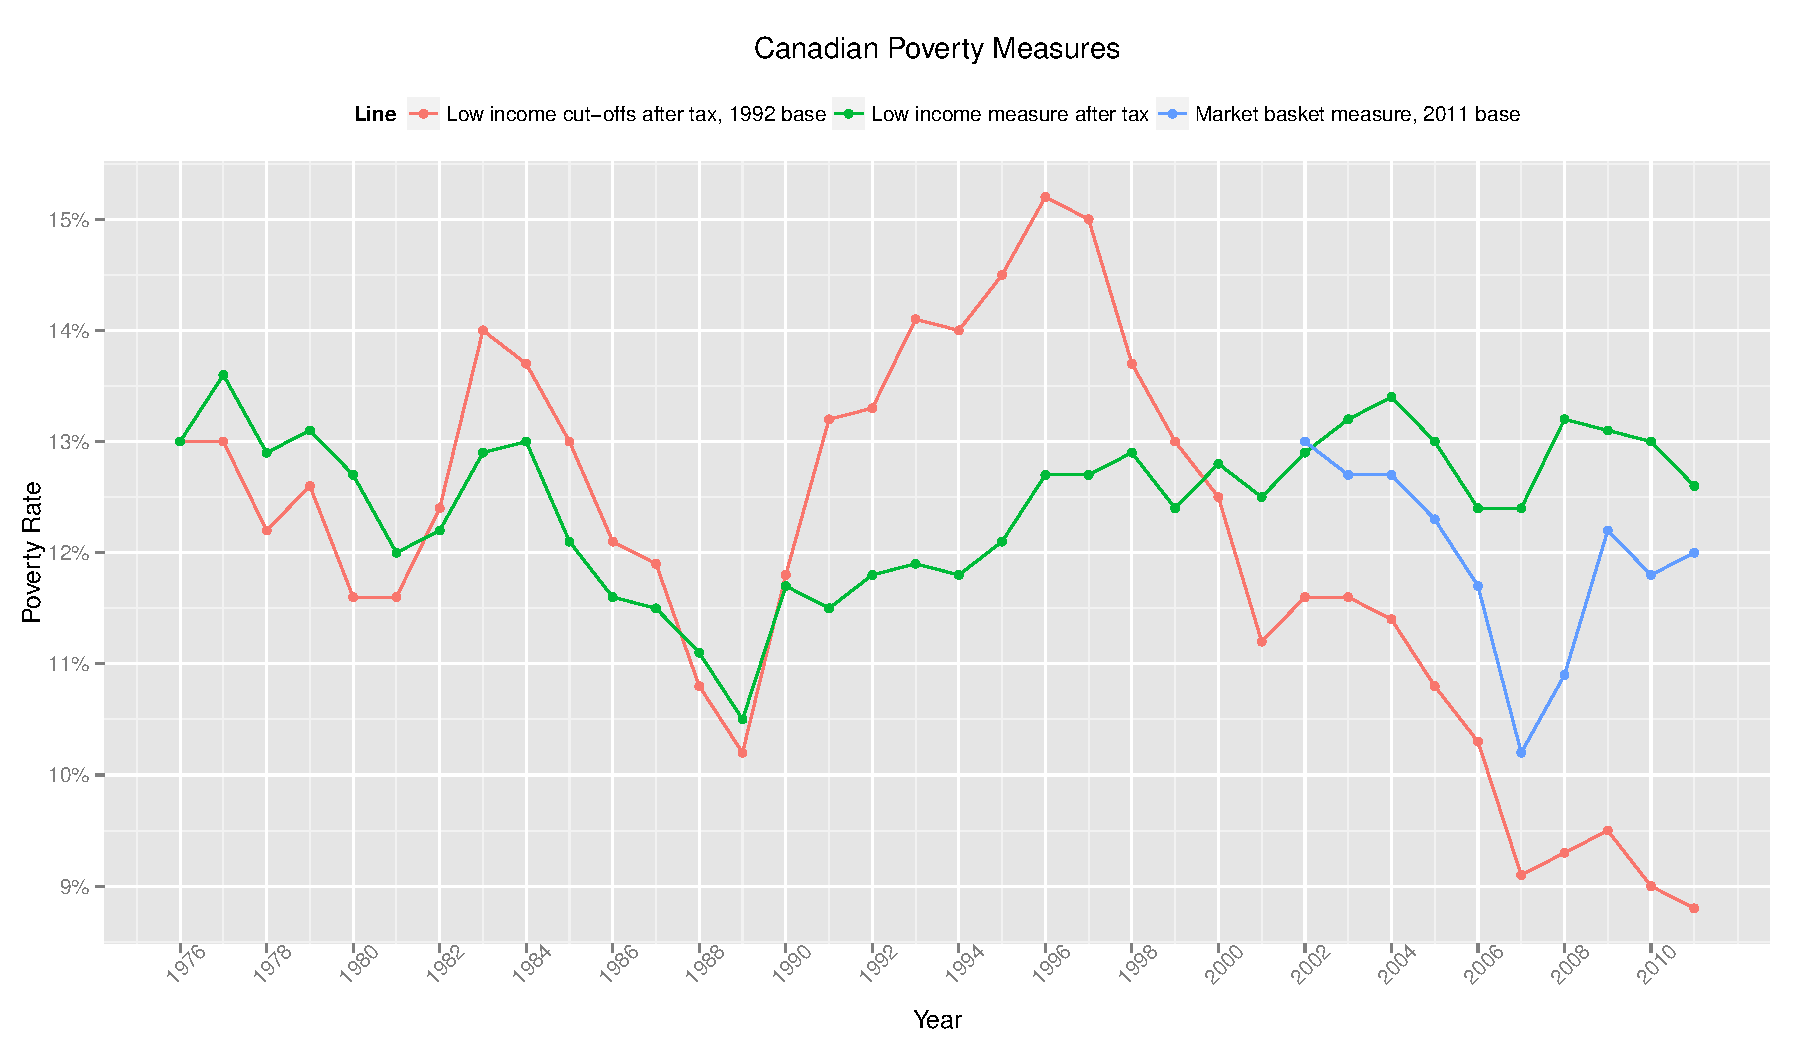
\includegraphics[width=\maxwidth]{figure/unnamed-chunk-2} 

\end{knitrout}

\end{center}
\end{figure}
\begin{figure}[ht]
\begin{center}
\begin{knitrout}
\definecolor{shadecolor}{rgb}{0.969, 0.969, 0.969}\color{fgcolor}
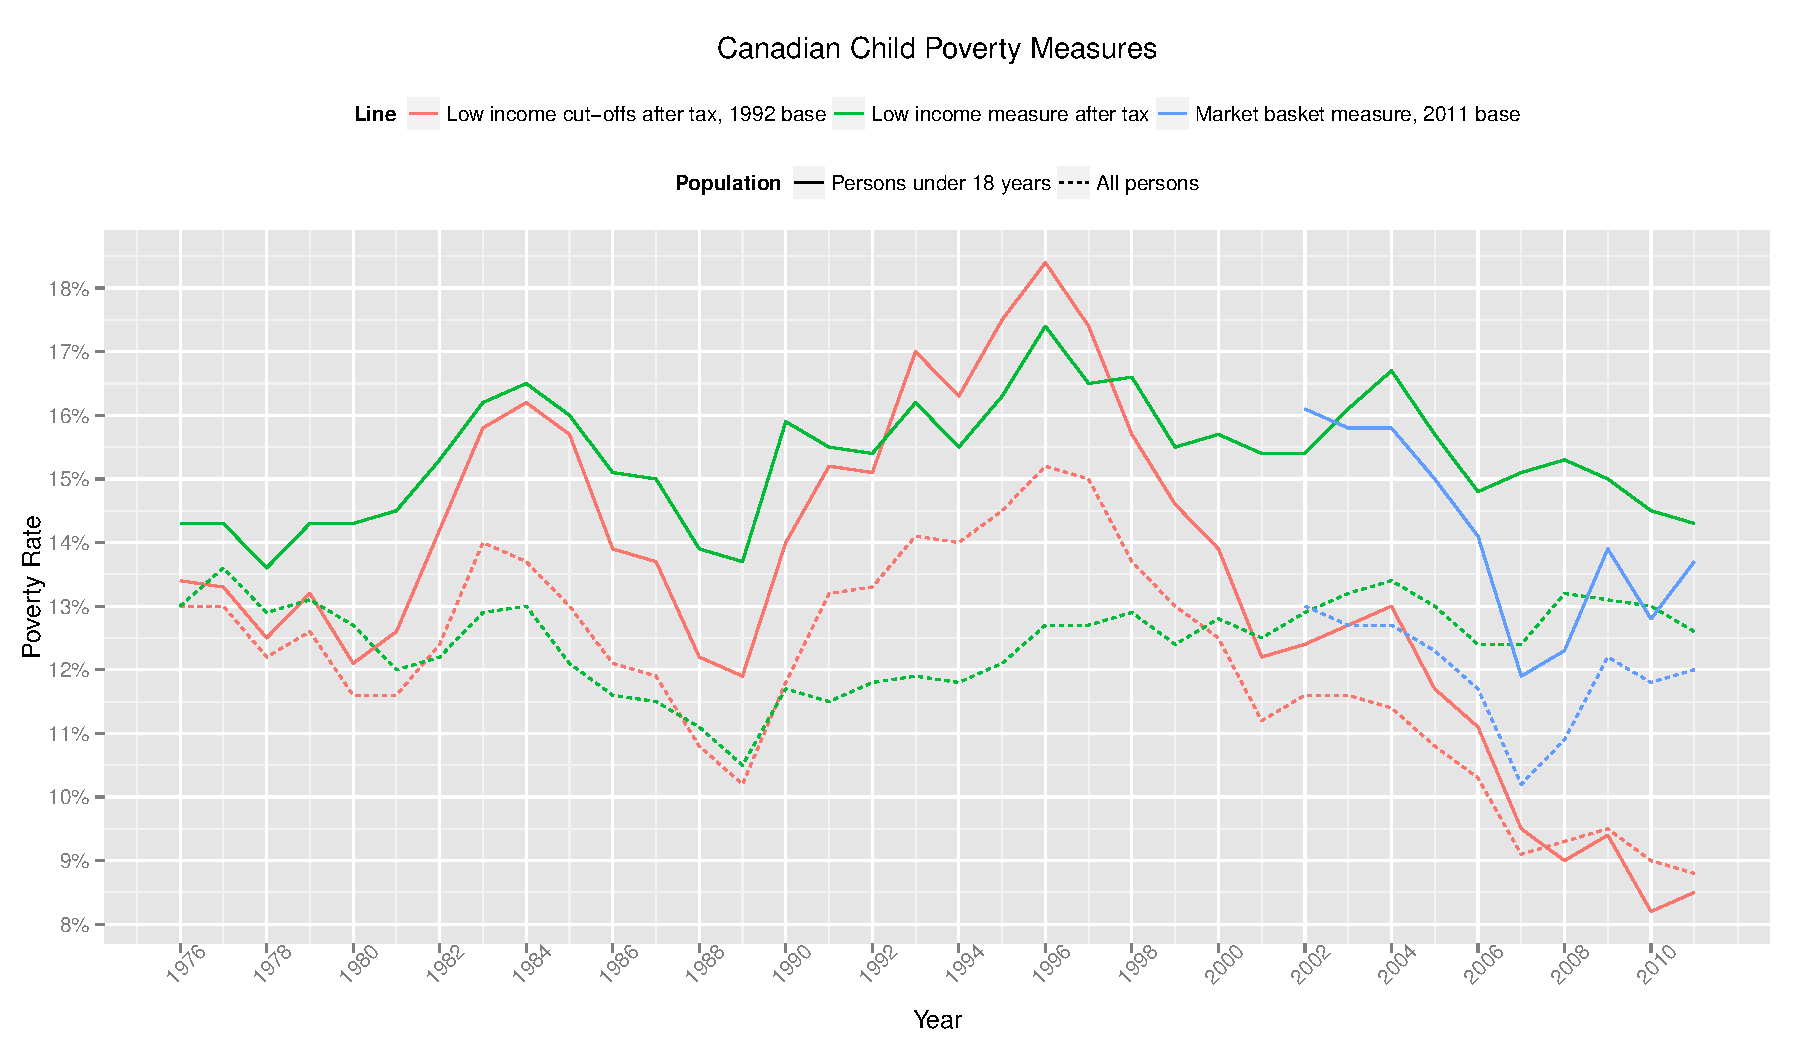
\includegraphics[width=\maxwidth]{figure/unnamed-chunk-3} 

\end{knitrout}

\end{center}
\end{figure}
\begin{figure}[ht]
\begin{center}
\begin{knitrout}
\definecolor{shadecolor}{rgb}{0.969, 0.969, 0.969}\color{fgcolor}
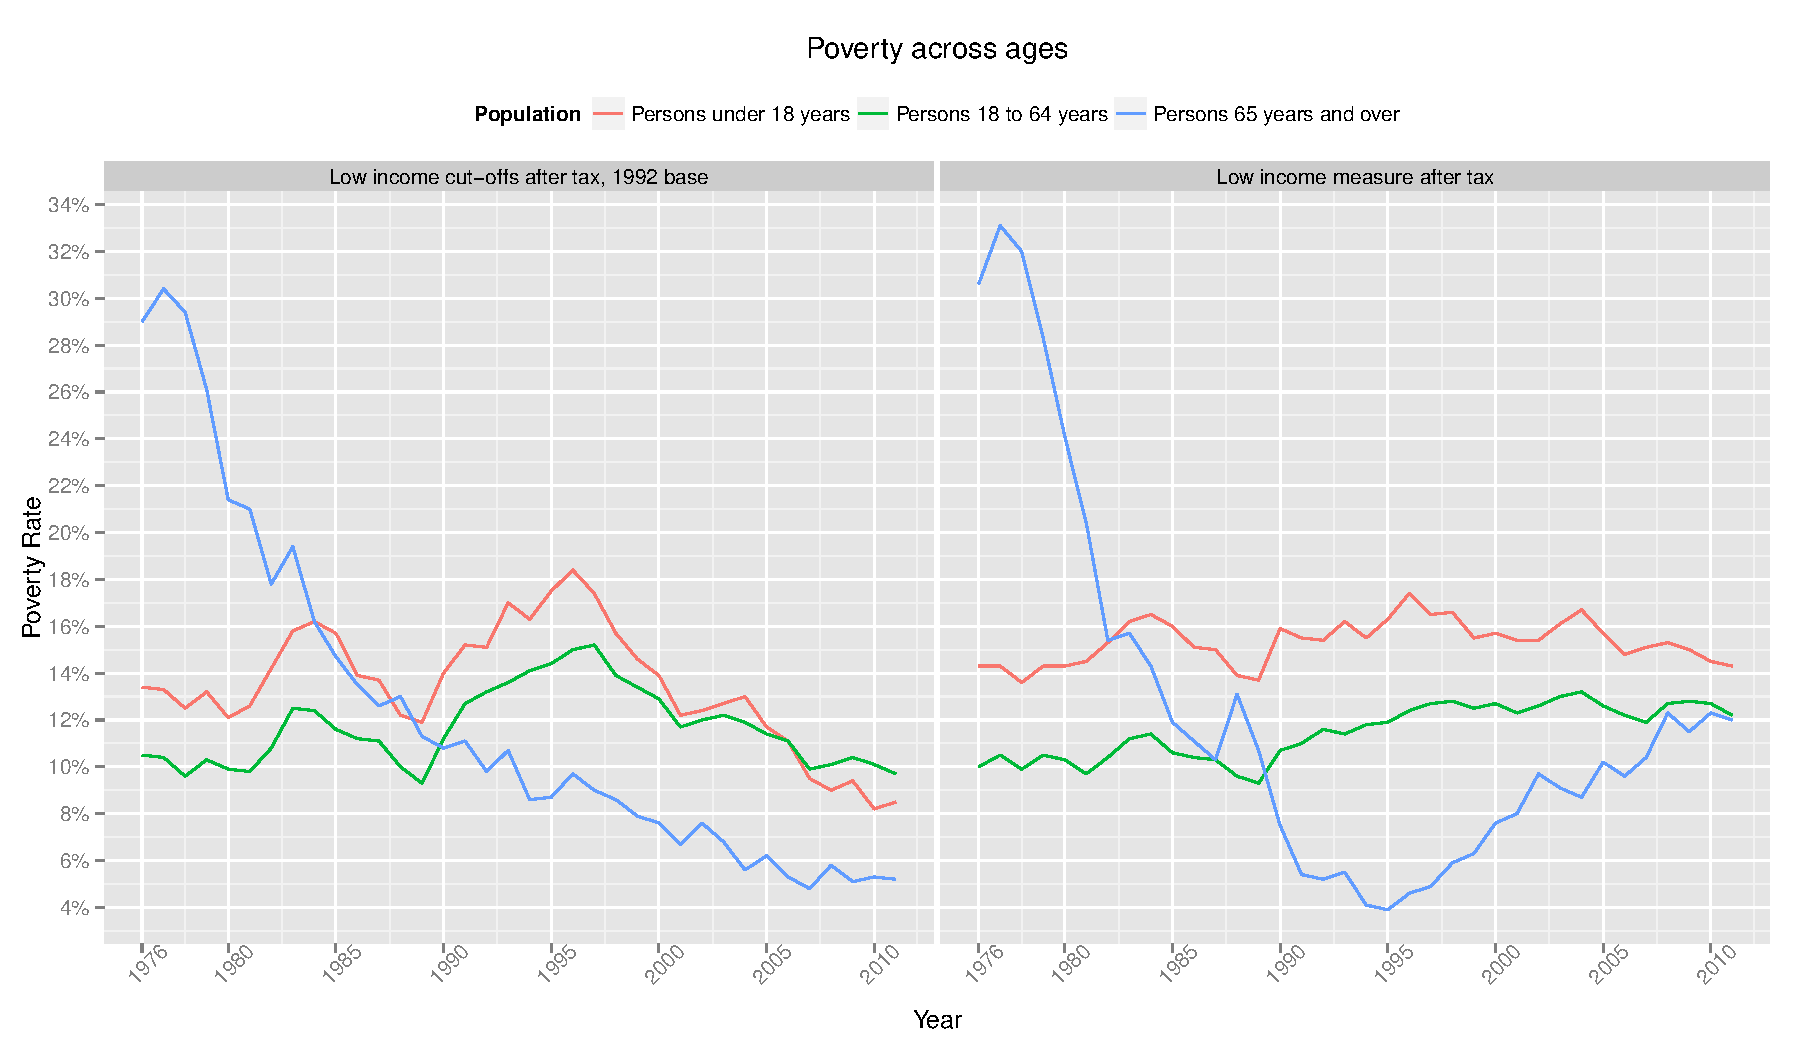
\includegraphics[width=\maxwidth]{figure/unnamed-chunk-4} 

\end{knitrout}

\end{center}
\end{figure}
\begin{figure}[ht]
\begin{center}
\begin{knitrout}
\definecolor{shadecolor}{rgb}{0.969, 0.969, 0.969}\color{fgcolor}
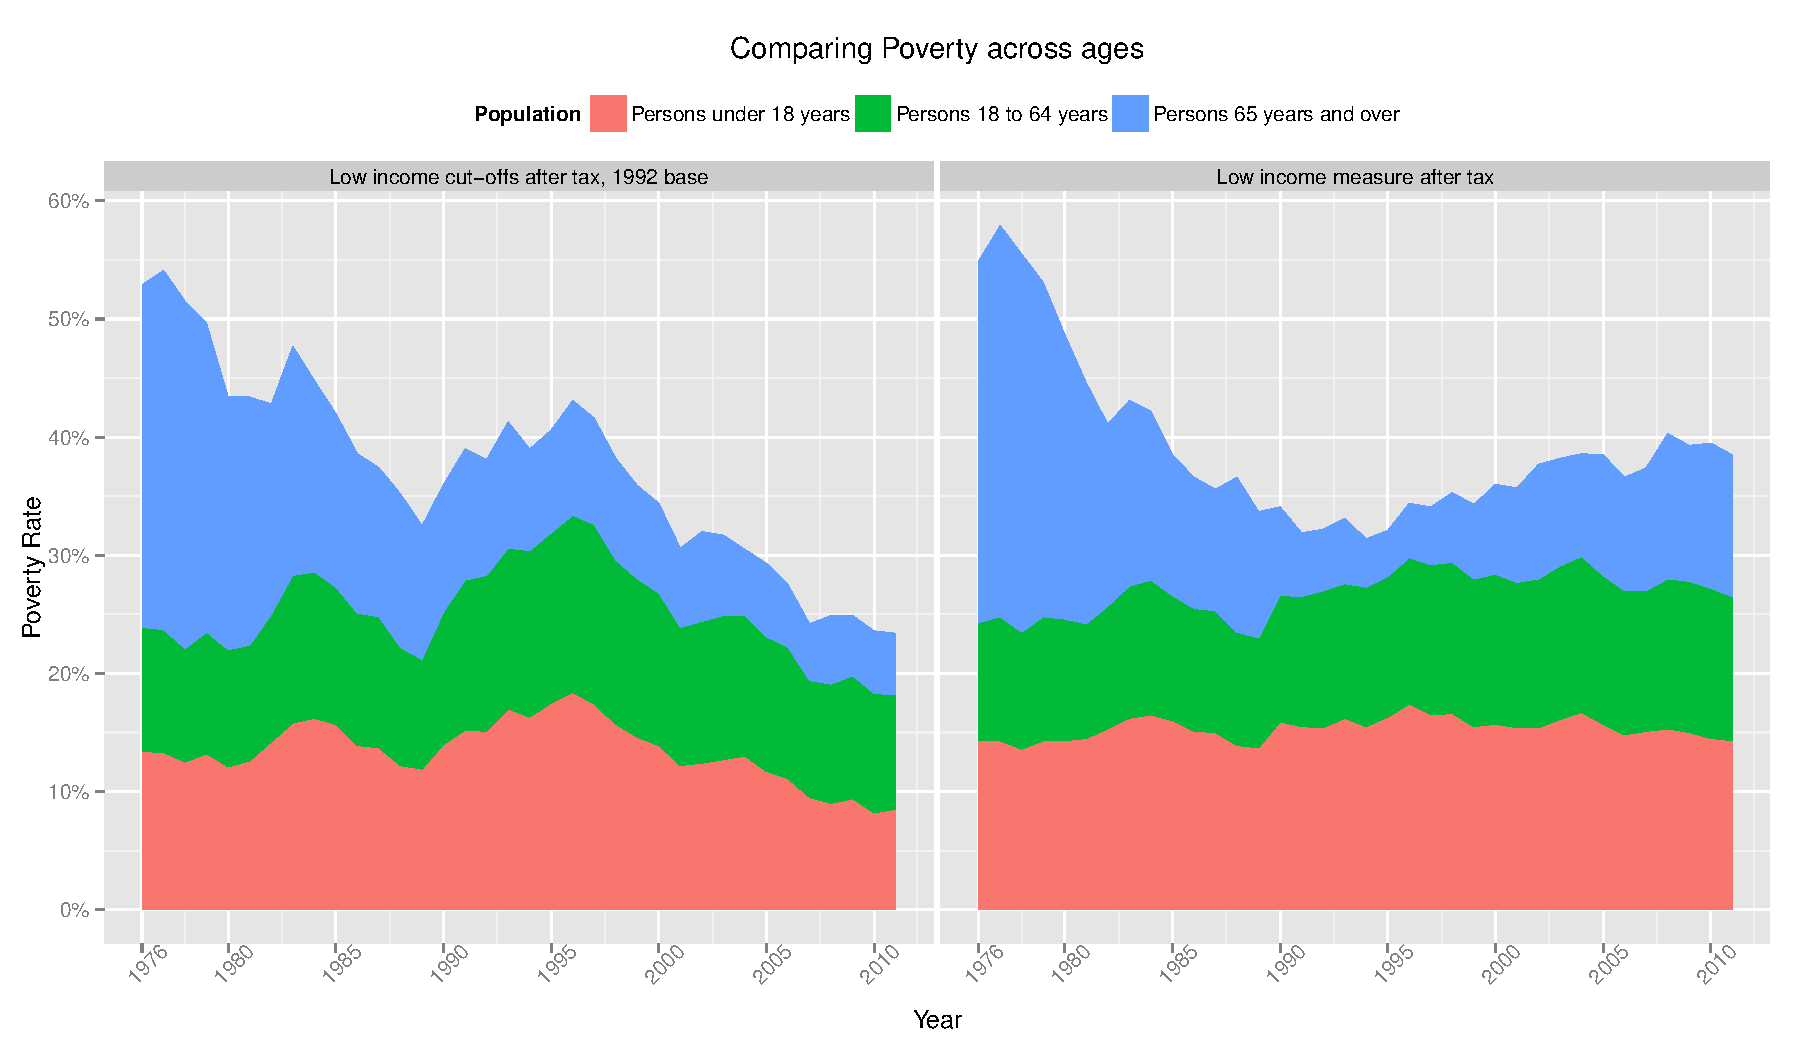
\includegraphics[width=\maxwidth]{figure/unnamed-chunk-5} 

\end{knitrout}

\end{center}
\end{figure}
\begin{figure}[ht]
\begin{center}
\begin{knitrout}
\definecolor{shadecolor}{rgb}{0.969, 0.969, 0.969}\color{fgcolor}
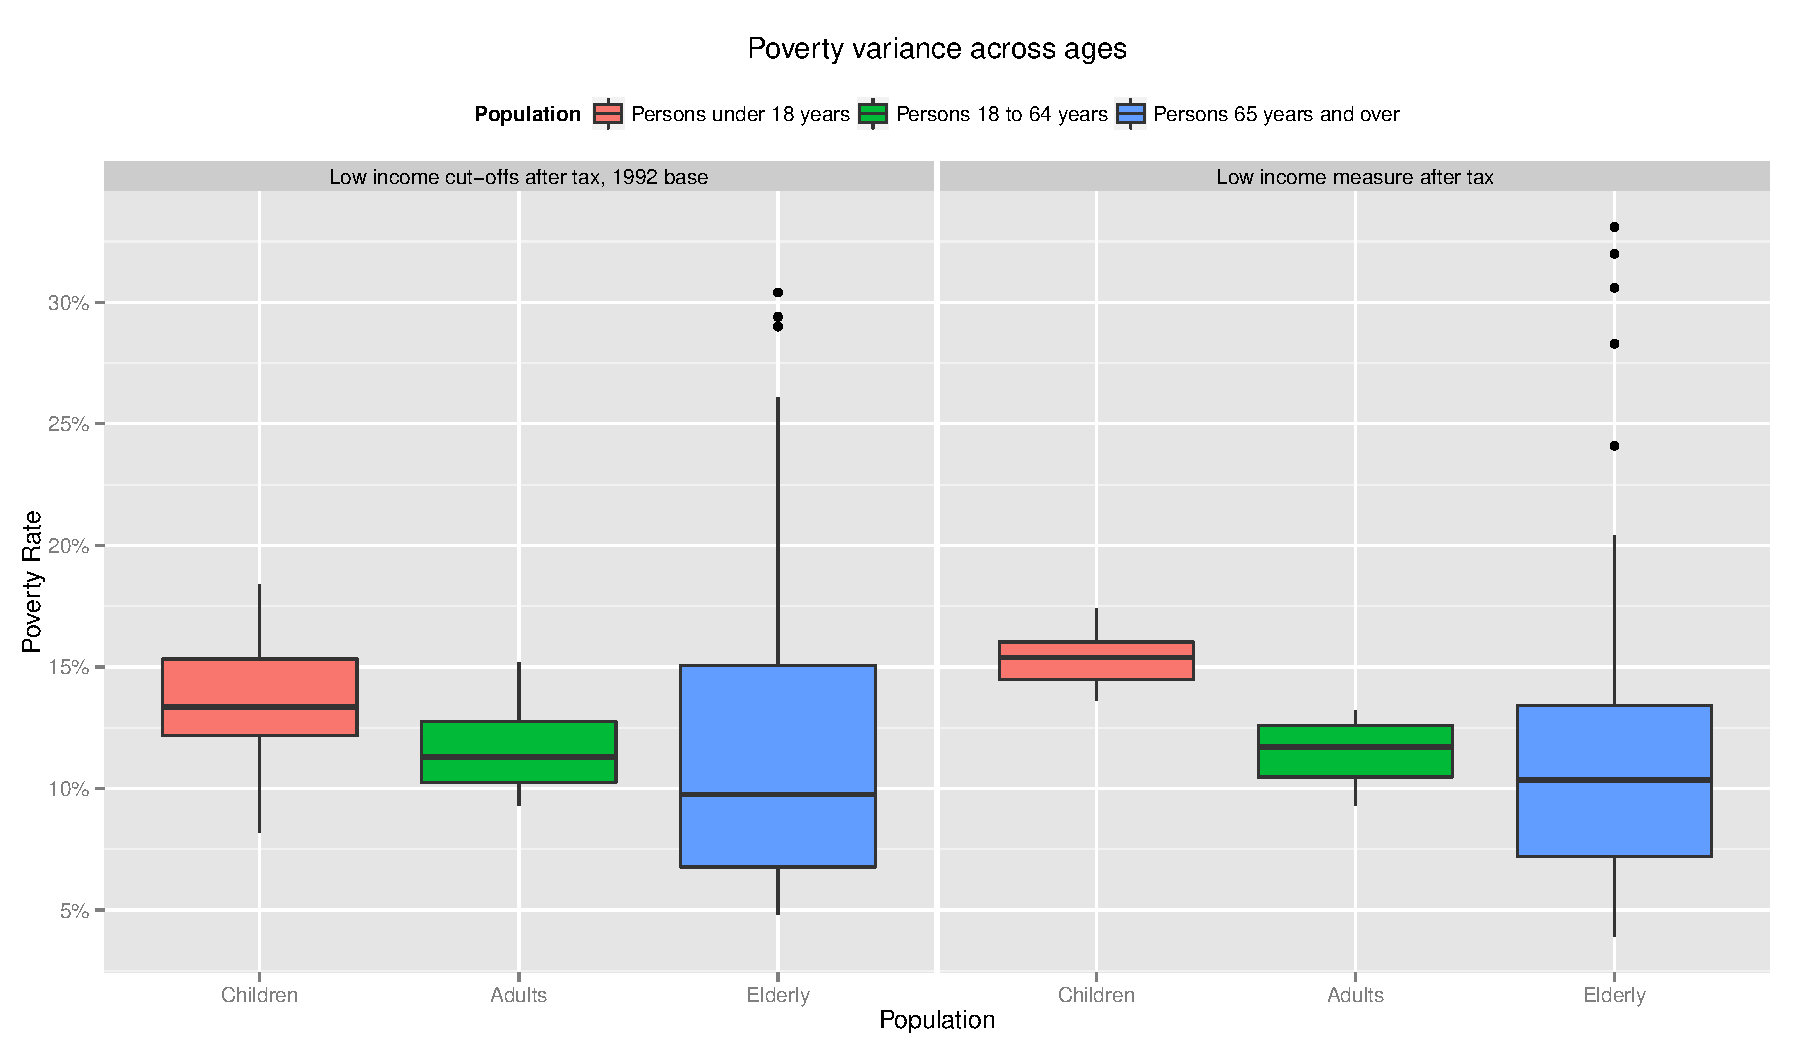
\includegraphics[width=\maxwidth]{figure/unnamed-chunk-6} 

\end{knitrout}

\end{center}
\end{figure}
\begin{figure}[ht]
\begin{center}
\begin{knitrout}
\definecolor{shadecolor}{rgb}{0.969, 0.969, 0.969}\color{fgcolor}
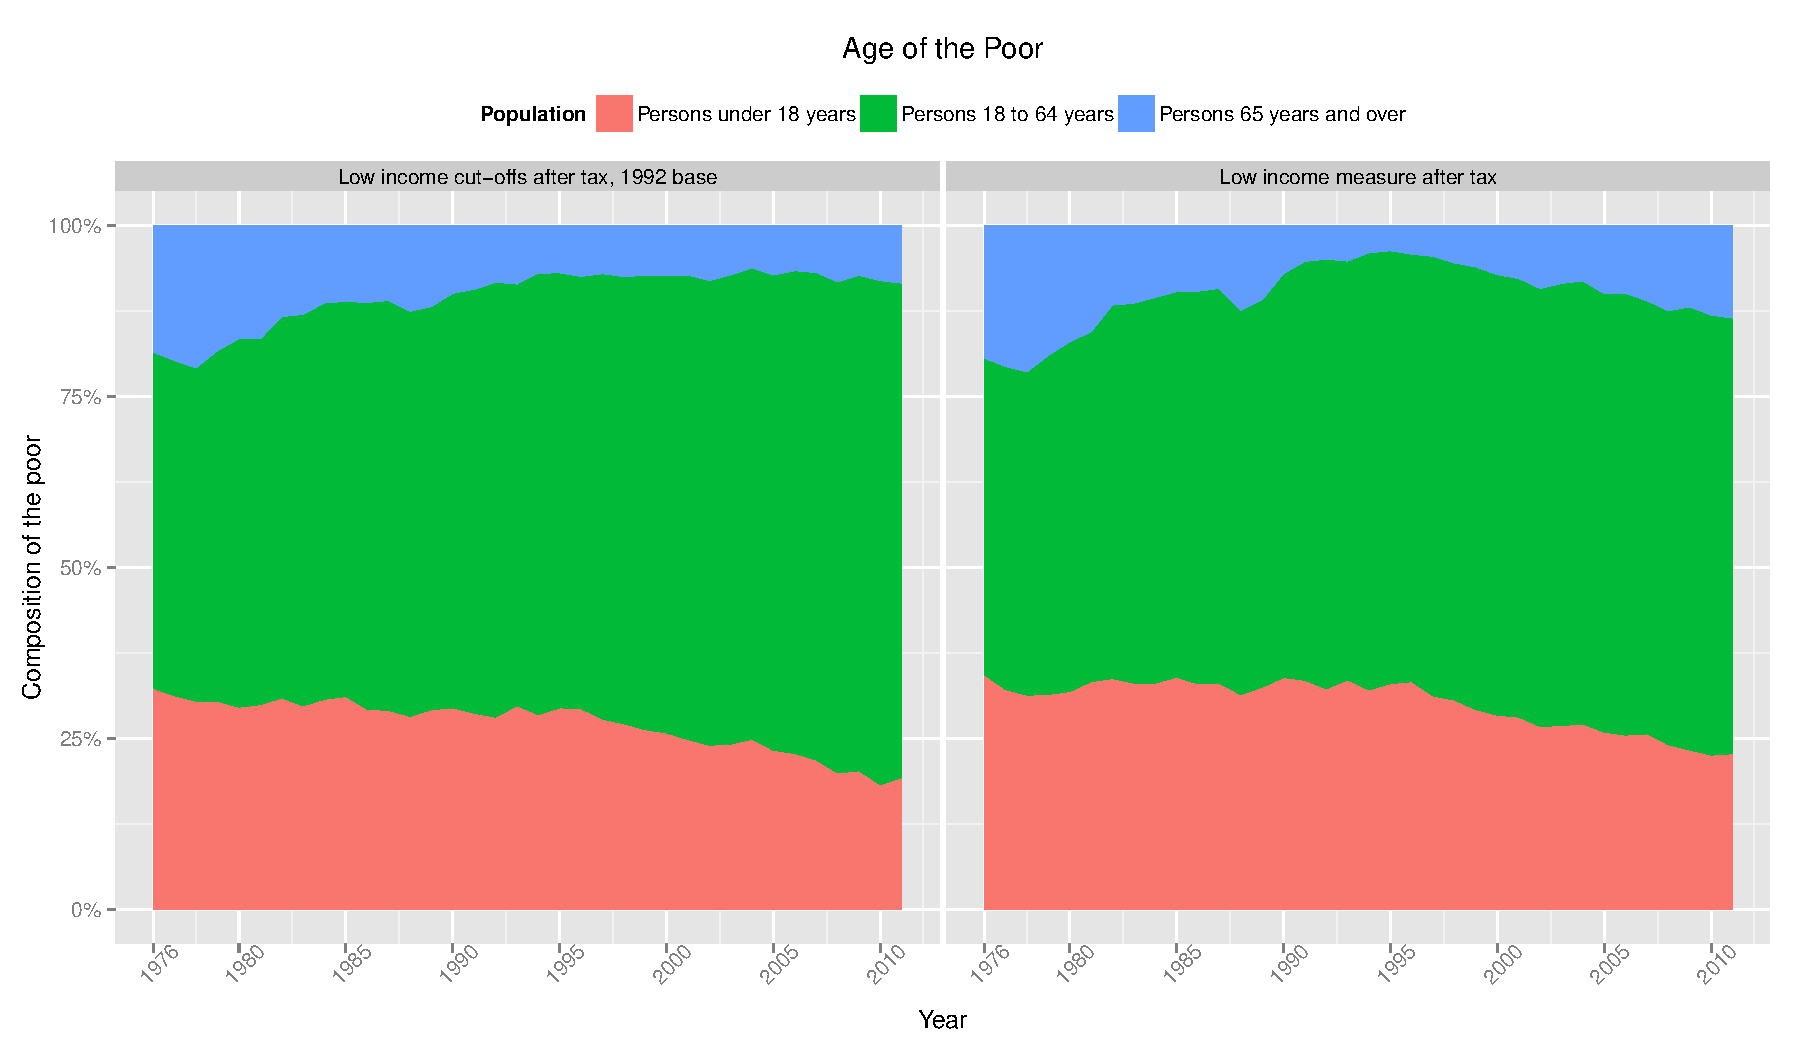
\includegraphics[width=\maxwidth]{figure/unnamed-chunk-7} 

\end{knitrout}

\end{center}
\end{figure}
\begin{figure}[ht]
\begin{center}
\begin{knitrout}
\definecolor{shadecolor}{rgb}{0.969, 0.969, 0.969}\color{fgcolor}
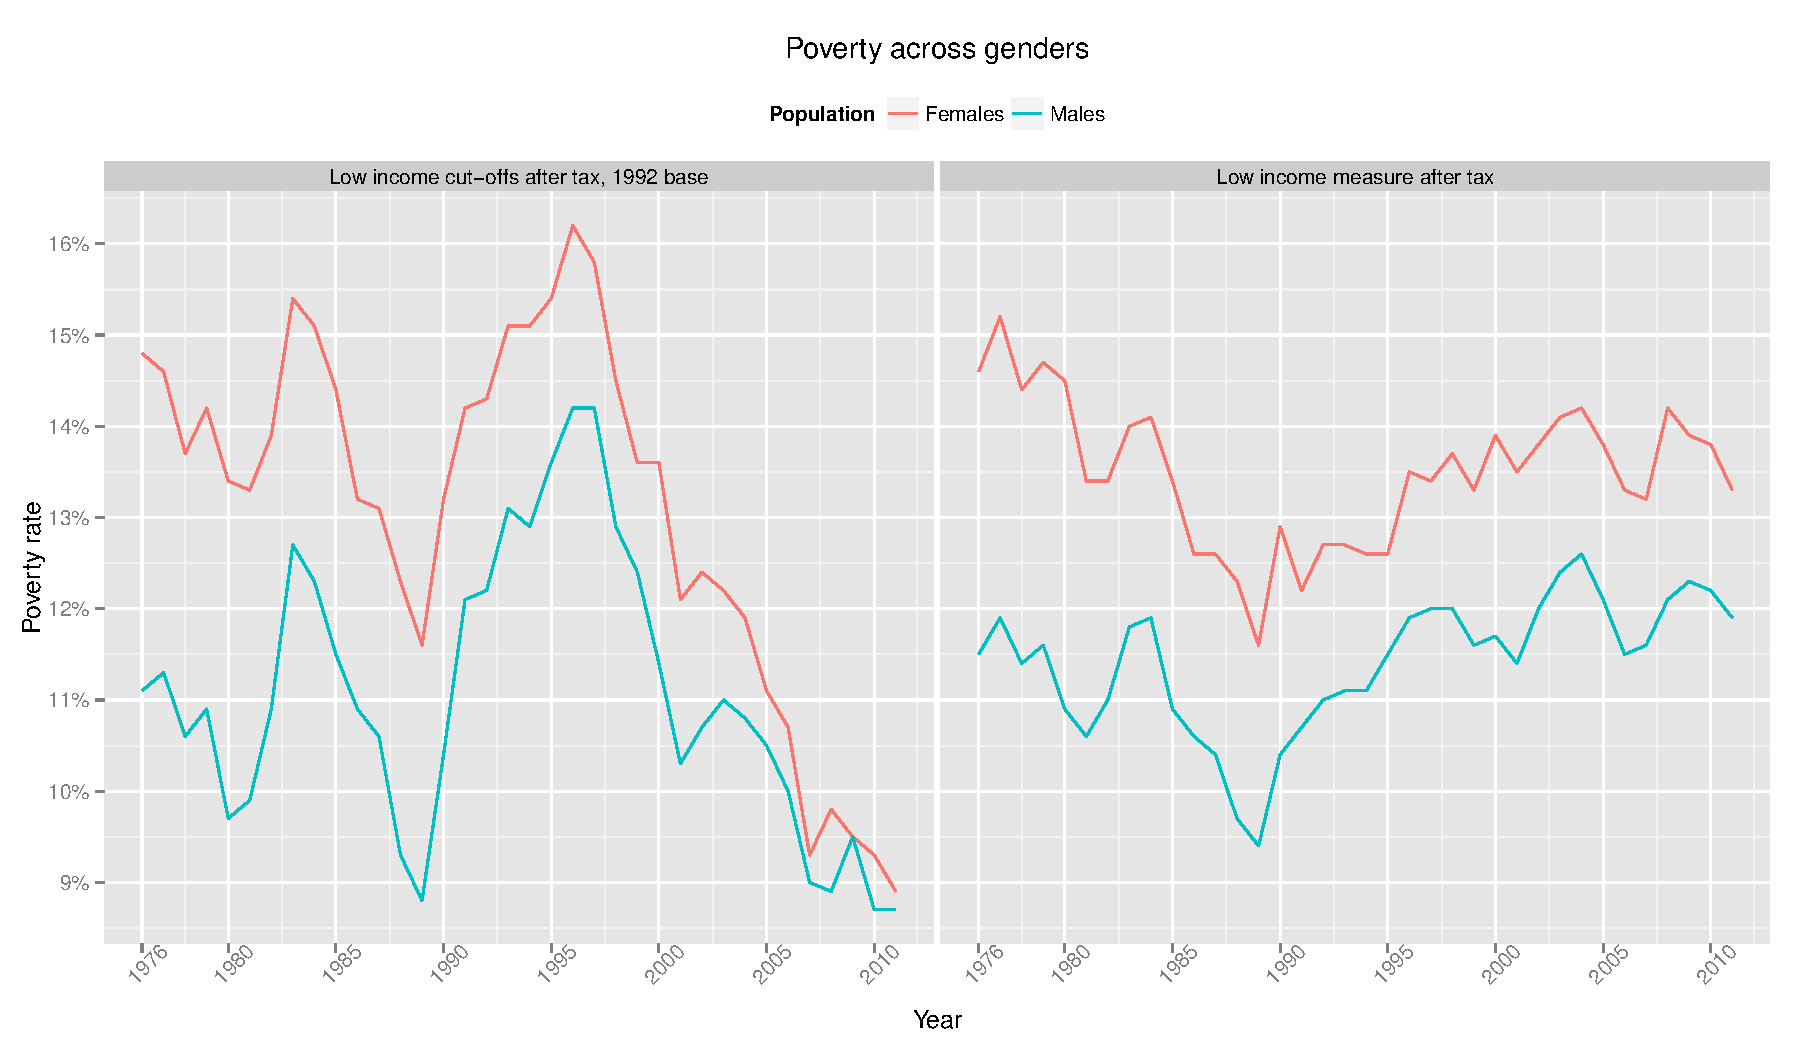
\includegraphics[width=\maxwidth]{figure/unnamed-chunk-8} 

\end{knitrout}

\end{center}
\end{figure}
\begin{figure}[ht]
\begin{center}
\begin{knitrout}
\definecolor{shadecolor}{rgb}{0.969, 0.969, 0.969}\color{fgcolor}
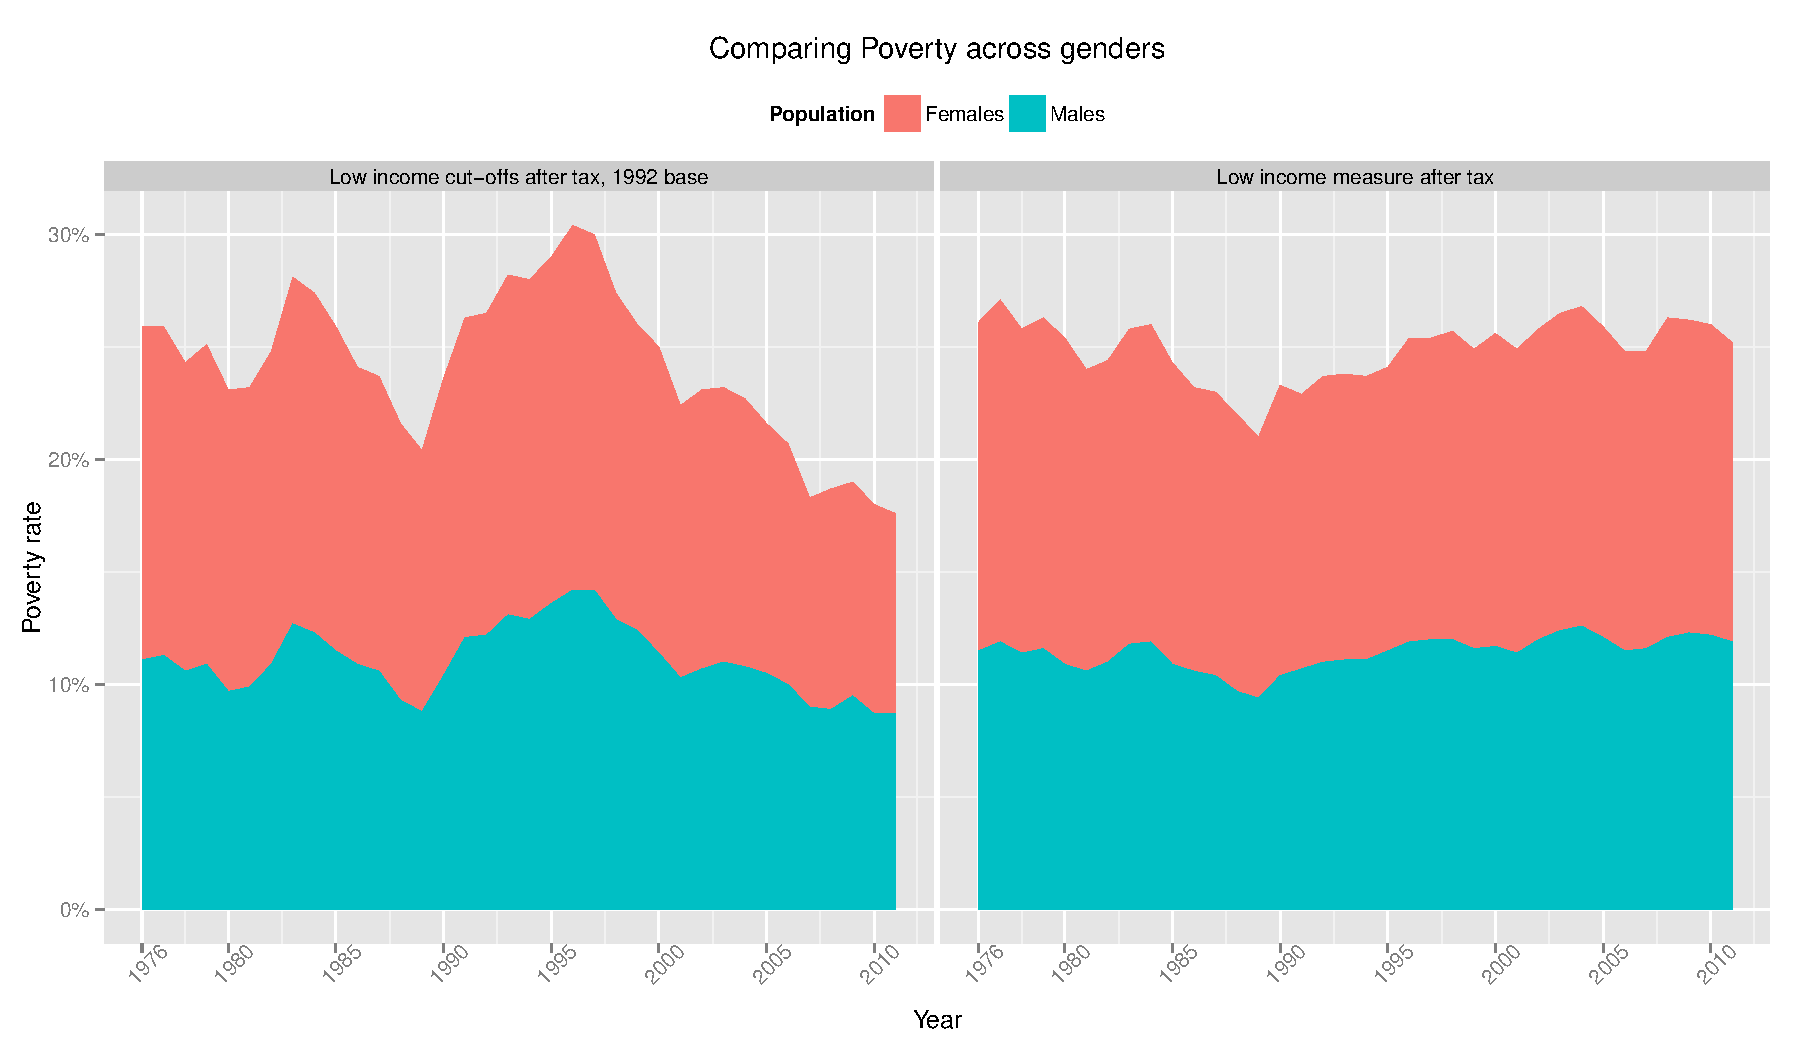
\includegraphics[width=\maxwidth]{figure/unnamed-chunk-9} 

\end{knitrout}

\end{center}
\end{figure}
\begin{figure}[ht]
\begin{center}
\begin{knitrout}
\definecolor{shadecolor}{rgb}{0.969, 0.969, 0.969}\color{fgcolor}
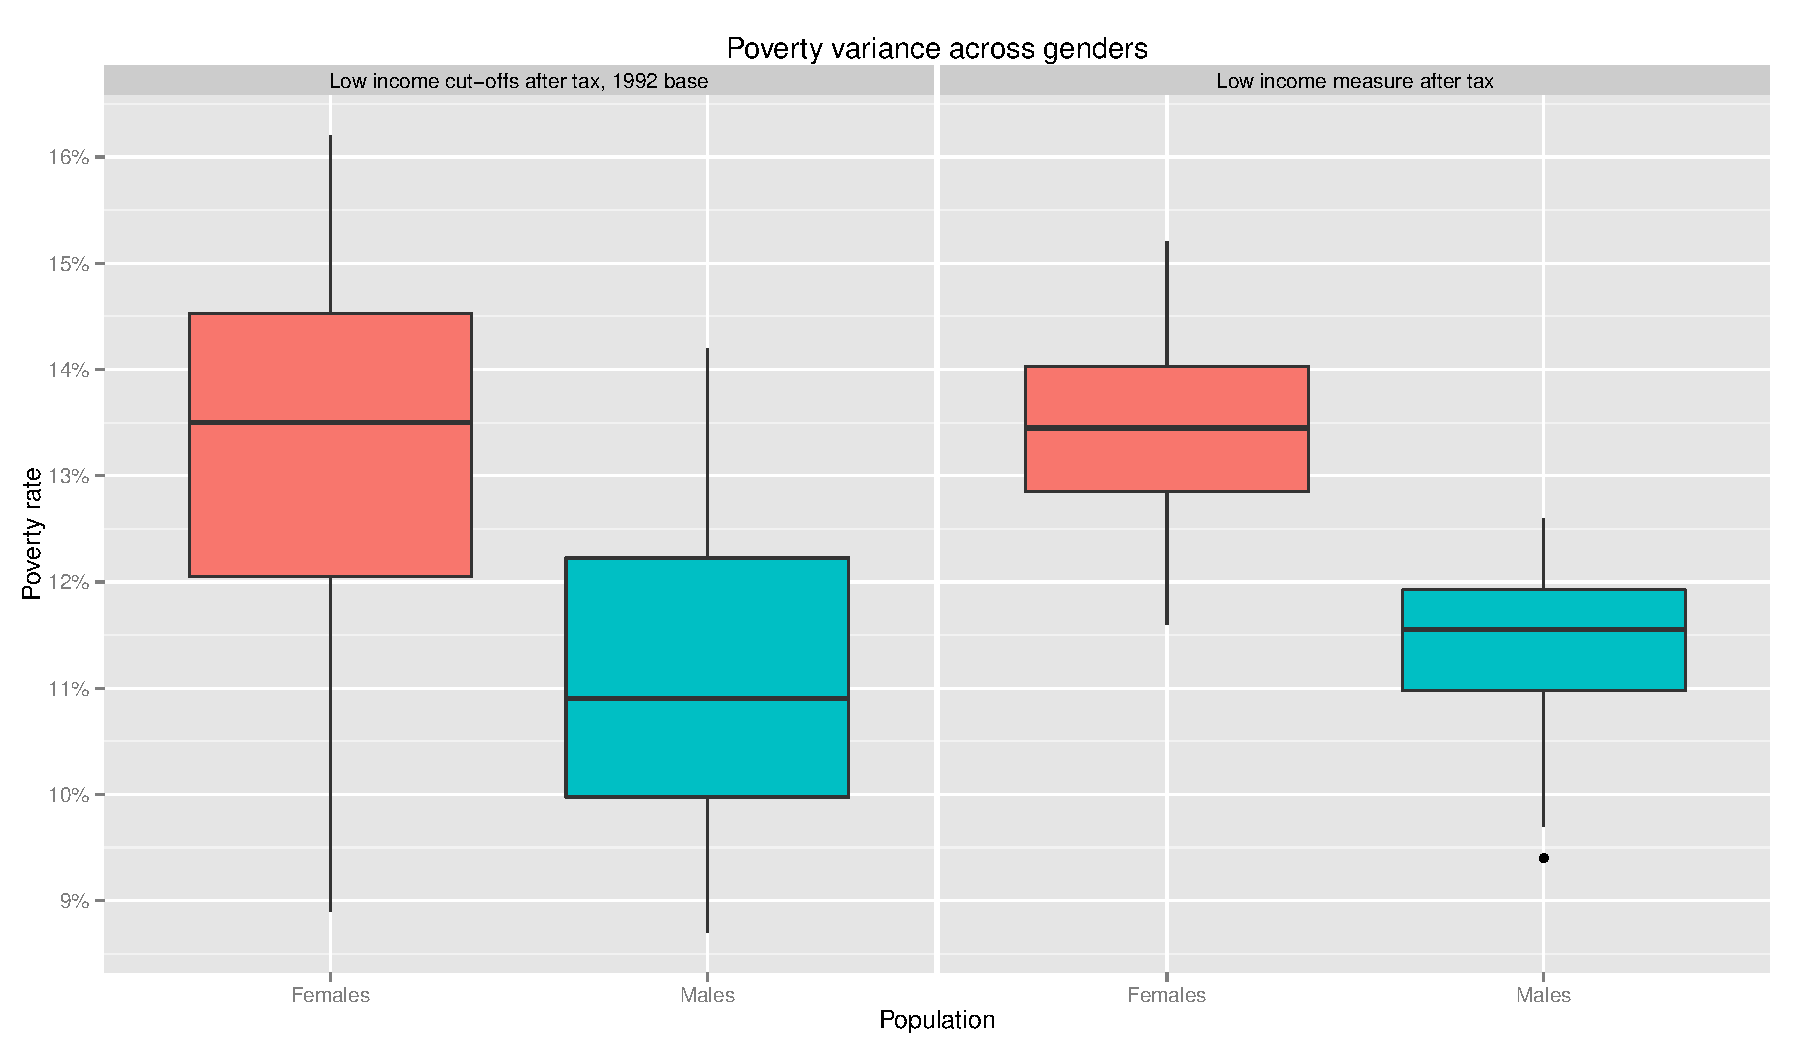
\includegraphics[width=\maxwidth]{figure/unnamed-chunk-10} 

\end{knitrout}

\end{center}
\end{figure}
\begin{figure}[ht]
\begin{center}
\begin{knitrout}
\definecolor{shadecolor}{rgb}{0.969, 0.969, 0.969}\color{fgcolor}
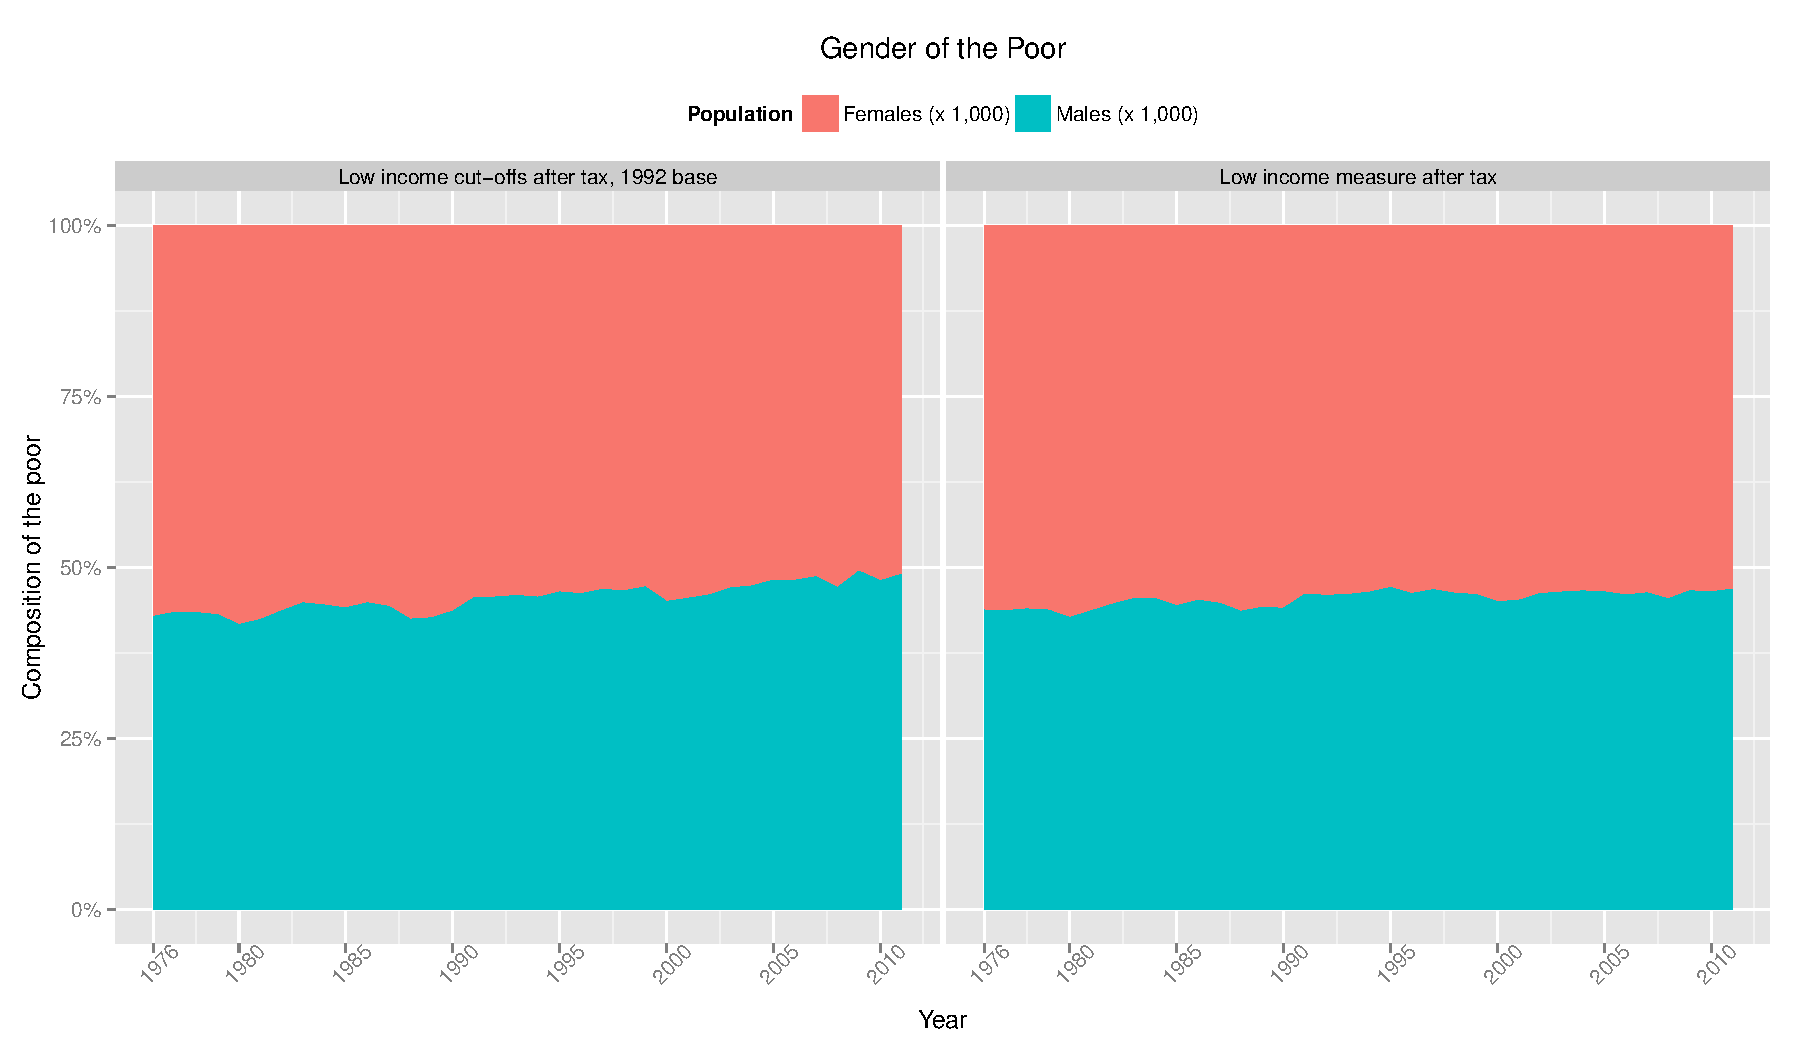
\includegraphics[width=\maxwidth]{figure/unnamed-chunk-11} 

\end{knitrout}

\end{center}
\end{figure}
\clearpage
\begin{figure}[ht]
\begin{center}
\begin{knitrout}
\definecolor{shadecolor}{rgb}{0.969, 0.969, 0.969}\color{fgcolor}
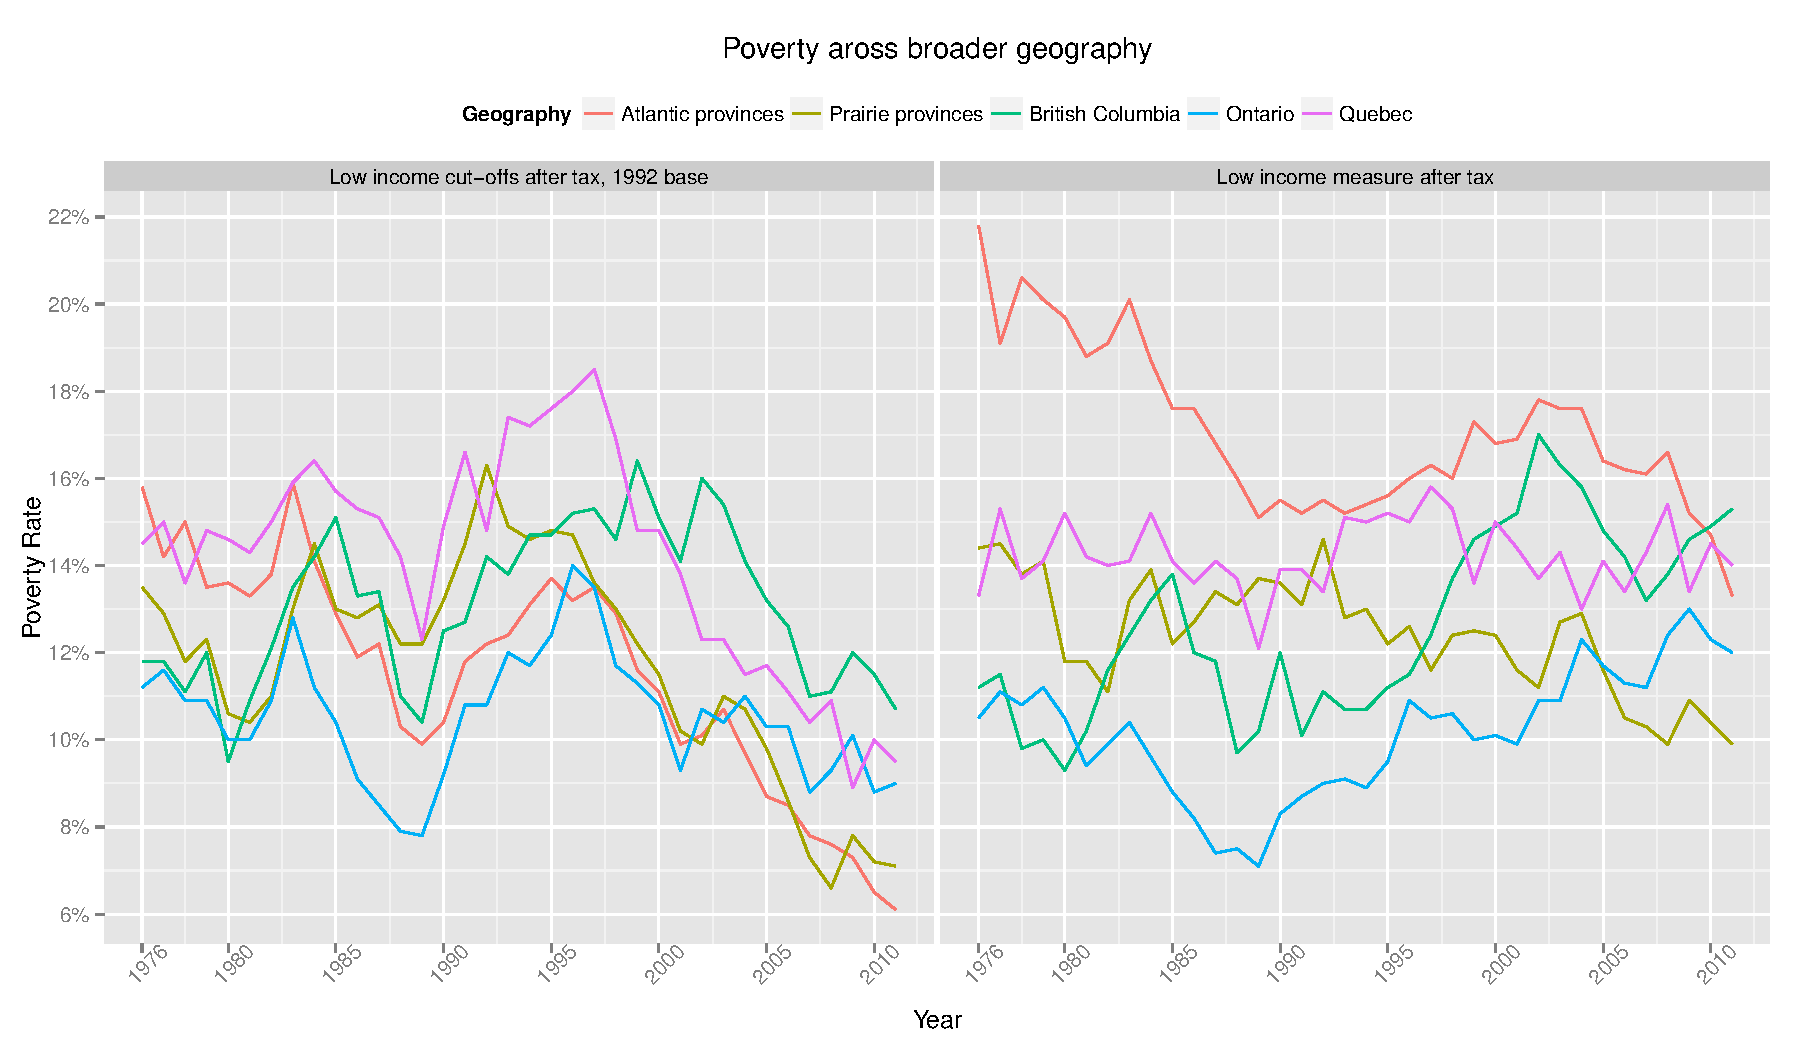
\includegraphics[width=\maxwidth]{figure/unnamed-chunk-12} 

\end{knitrout}

\end{center}
\end{figure}
\begin{figure}[ht]
\begin{center}
\begin{knitrout}
\definecolor{shadecolor}{rgb}{0.969, 0.969, 0.969}\color{fgcolor}
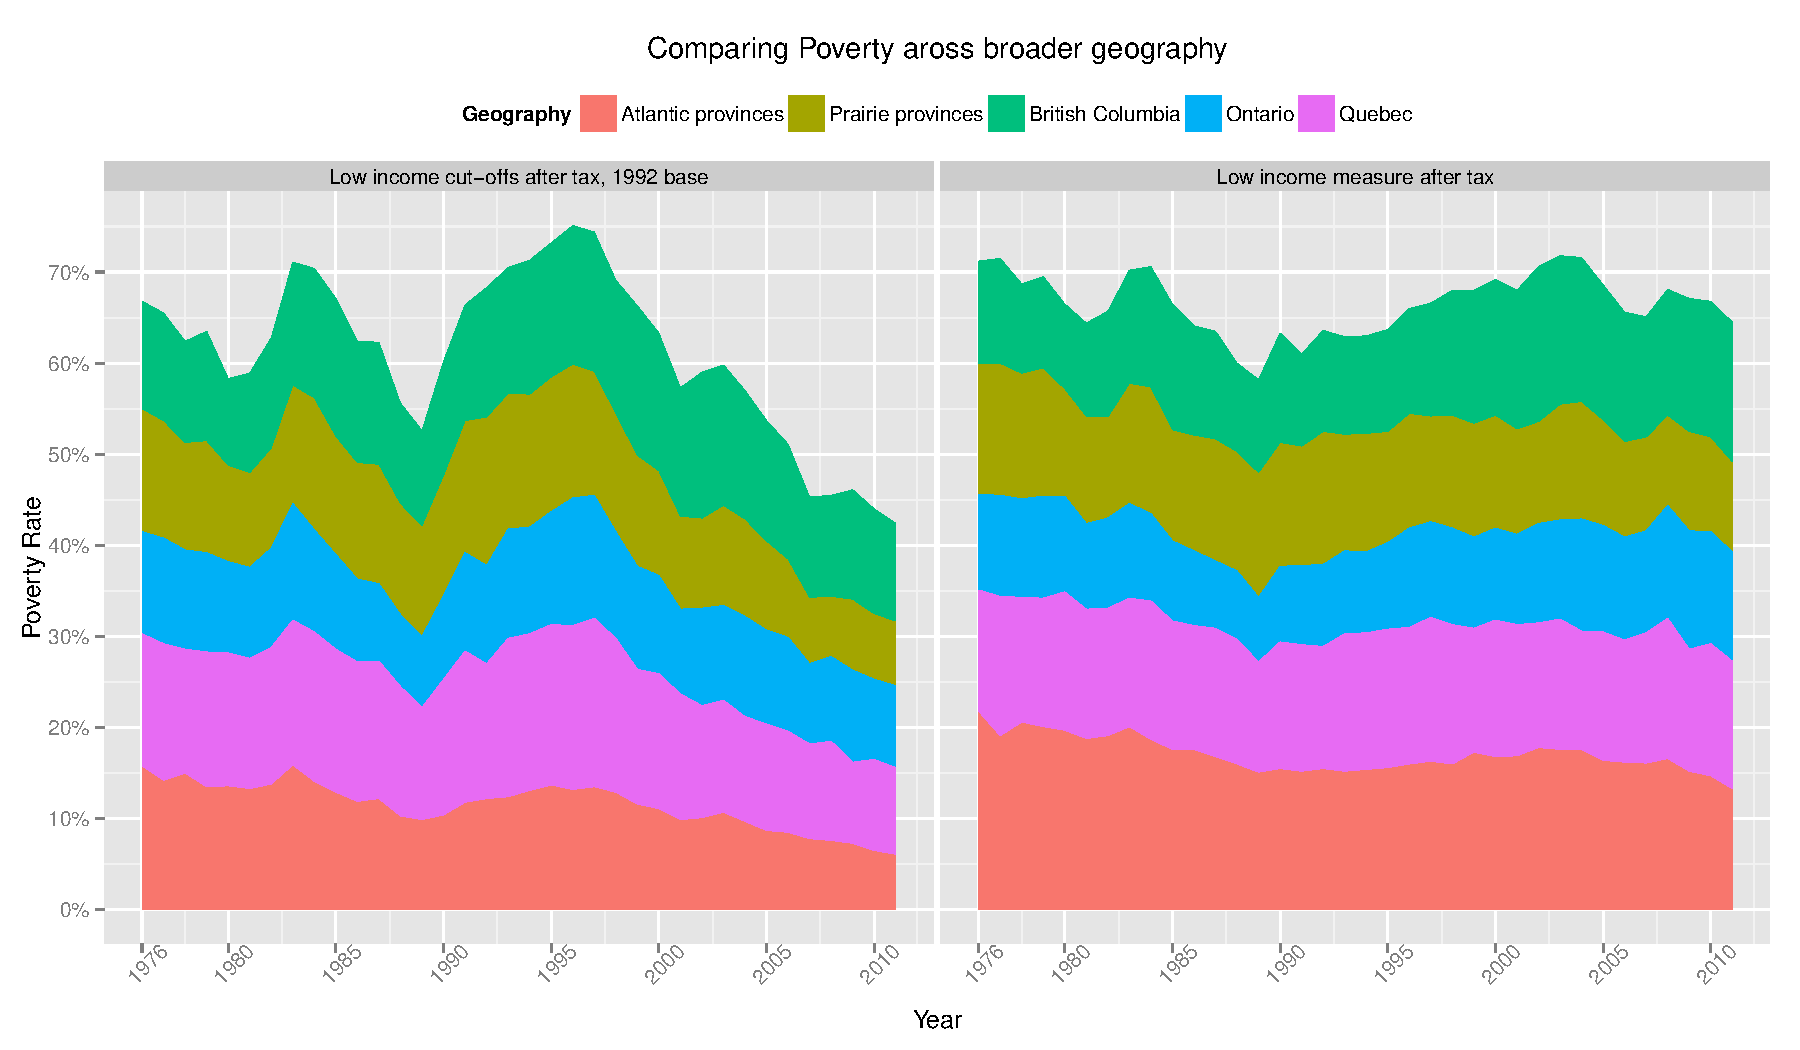
\includegraphics[width=\maxwidth]{figure/unnamed-chunk-13} 

\end{knitrout}

\end{center}
\end{figure}
\begin{figure}[ht]
\begin{center}
\begin{knitrout}
\definecolor{shadecolor}{rgb}{0.969, 0.969, 0.969}\color{fgcolor}
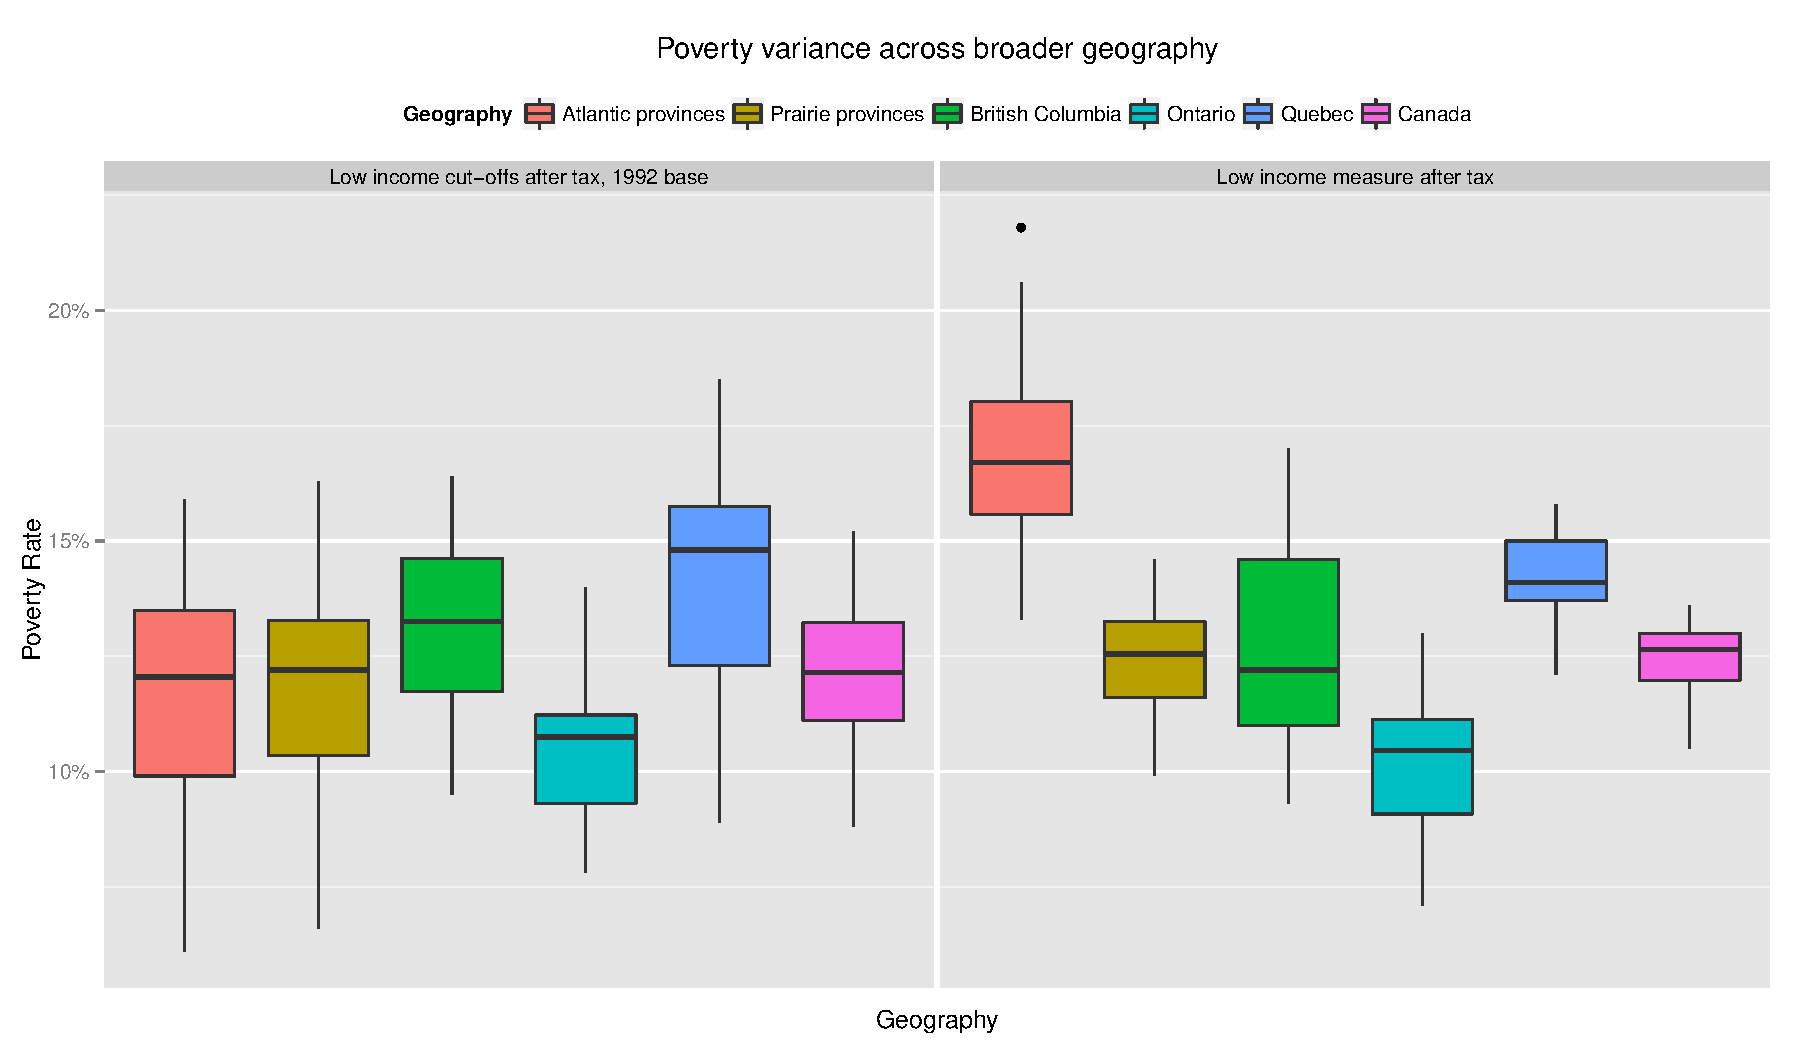
\includegraphics[width=\maxwidth]{figure/unnamed-chunk-14} 

\end{knitrout}

\end{center}
\end{figure}
\begin{figure}[ht]
\begin{center}
\begin{knitrout}
\definecolor{shadecolor}{rgb}{0.969, 0.969, 0.969}\color{fgcolor}
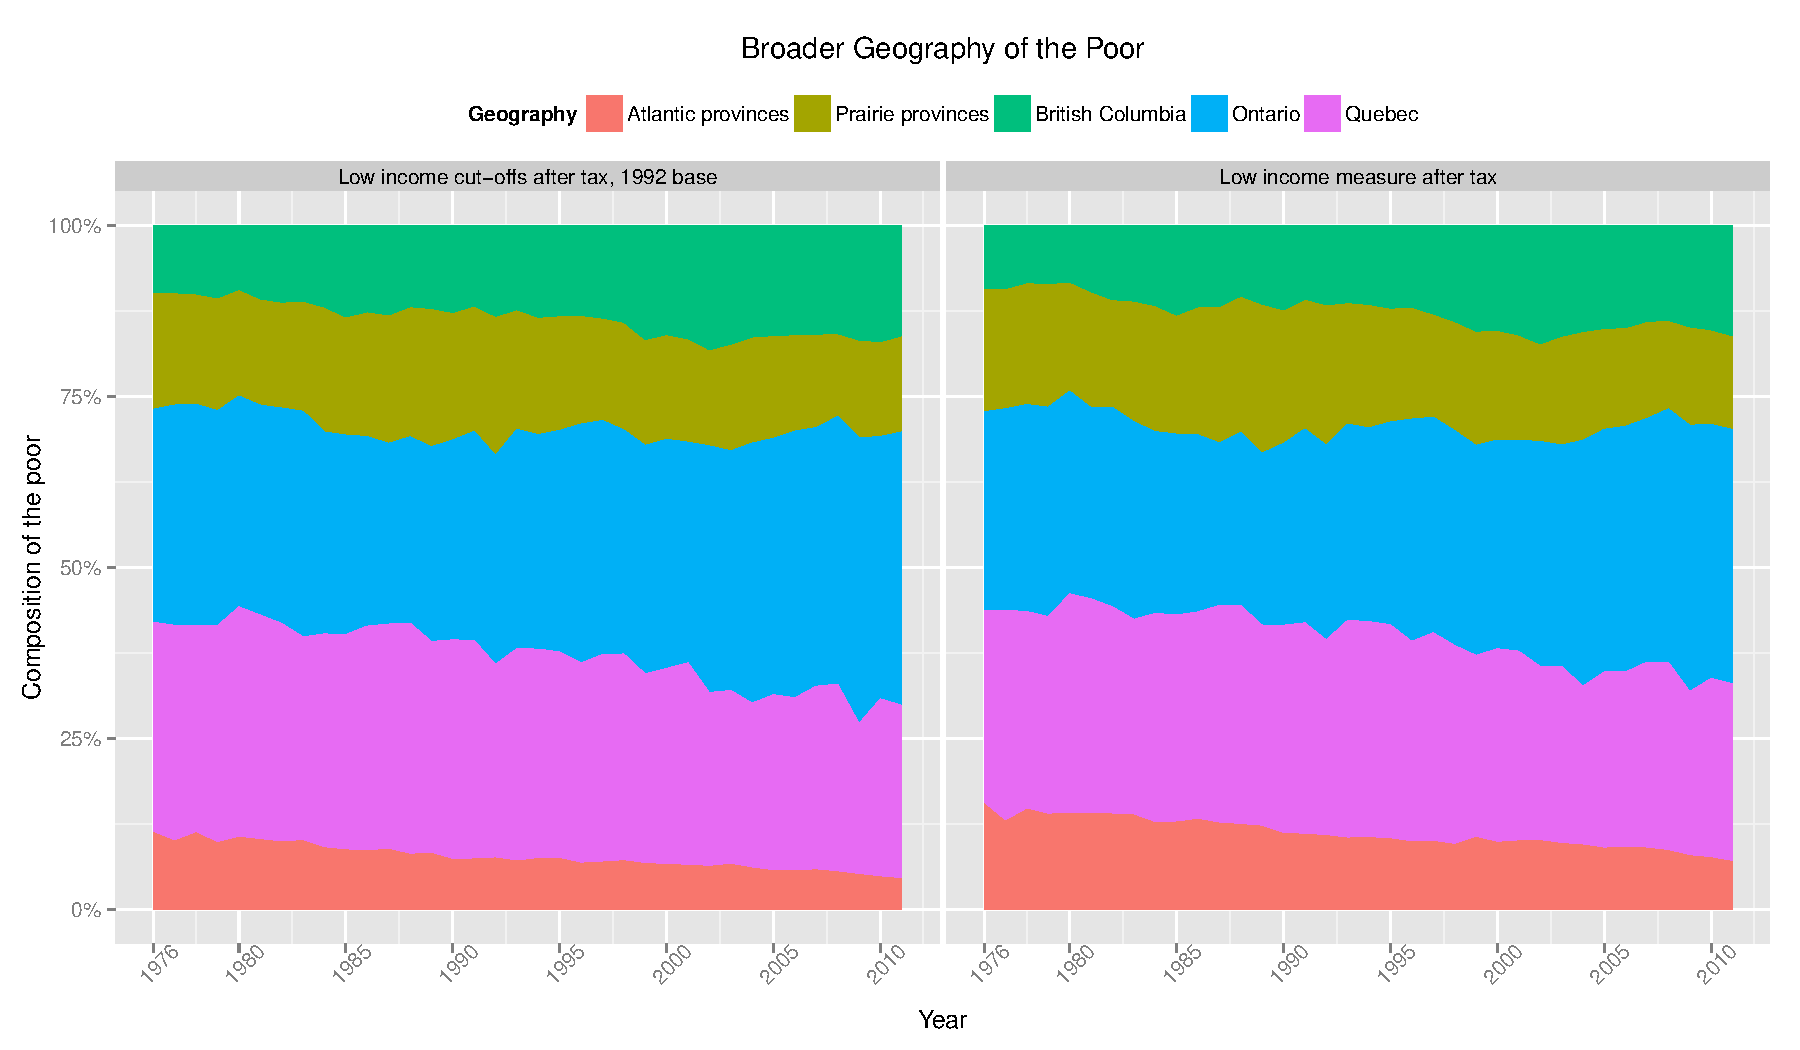
\includegraphics[width=\maxwidth]{figure/unnamed-chunk-15} 

\end{knitrout}

\end{center}
\end{figure}
\begin{figure}[ht]
\begin{center}
\begin{knitrout}
\definecolor{shadecolor}{rgb}{0.969, 0.969, 0.969}\color{fgcolor}
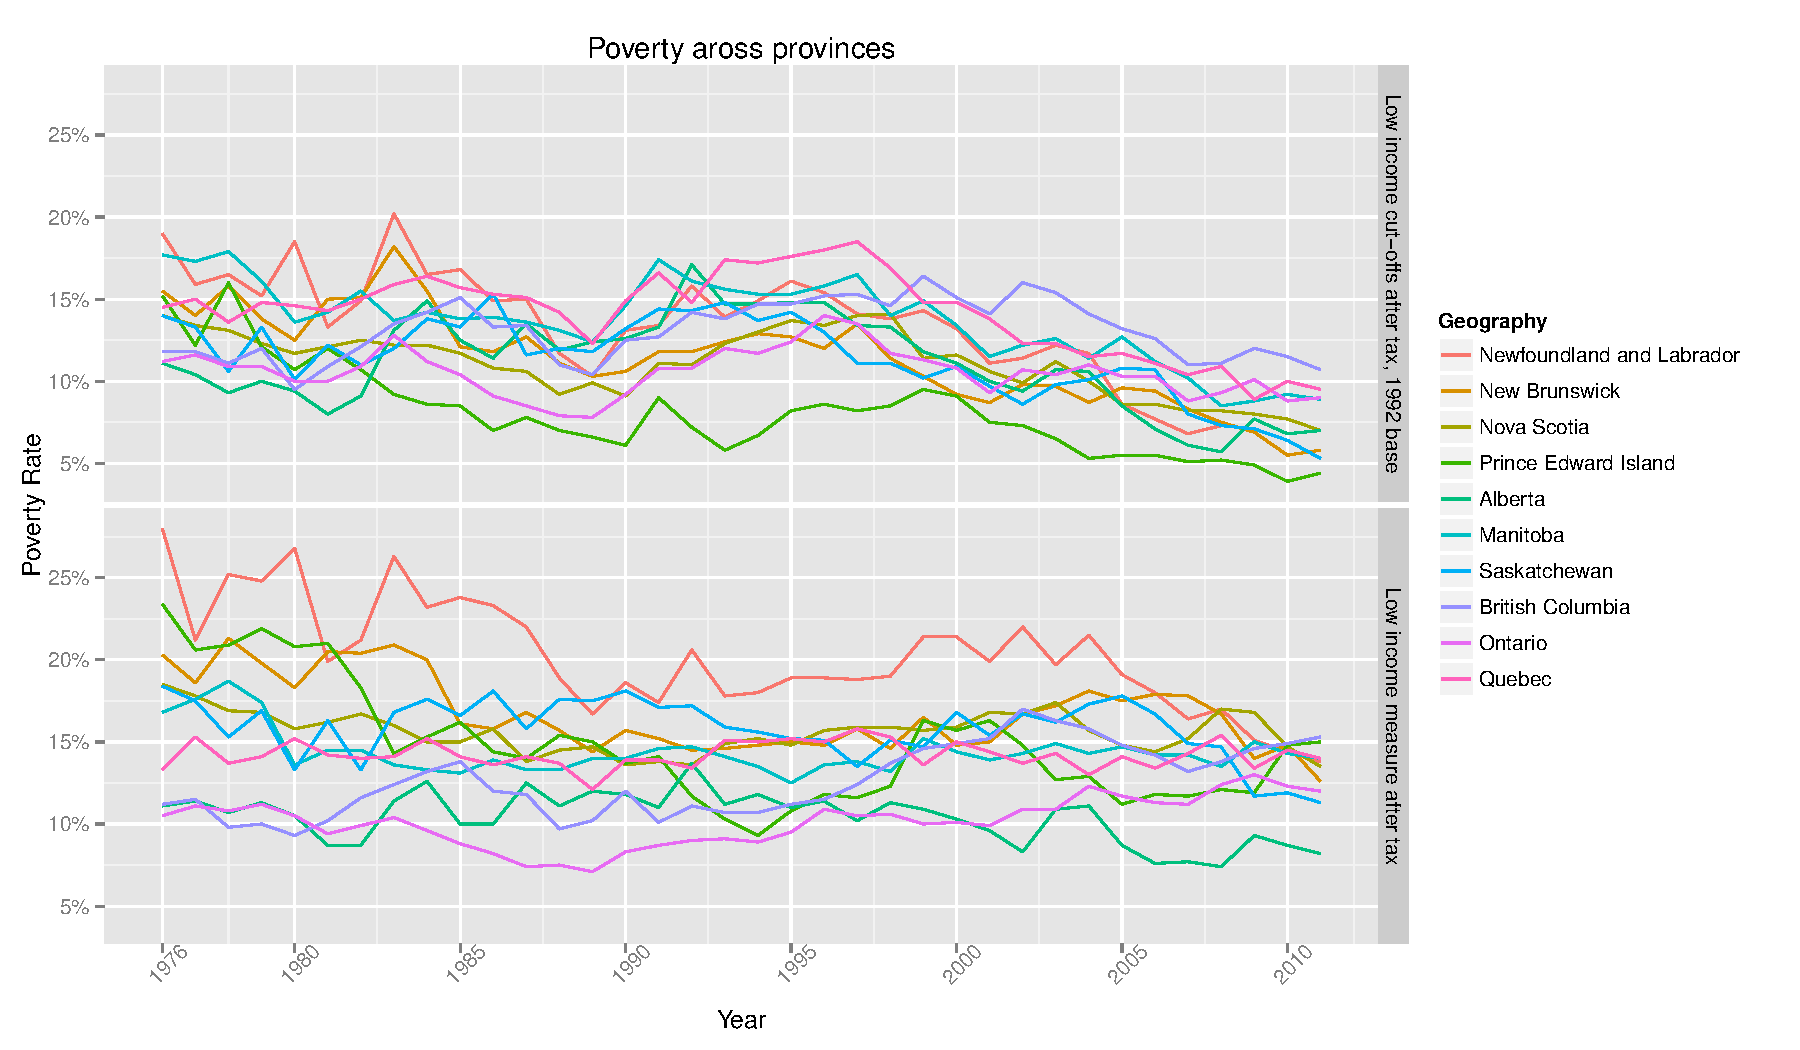
\includegraphics[width=\maxwidth]{figure/unnamed-chunk-16} 

\end{knitrout}

\end{center}
\end{figure}
\begin{figure}[ht]
\begin{center}
\begin{knitrout}
\definecolor{shadecolor}{rgb}{0.969, 0.969, 0.969}\color{fgcolor}
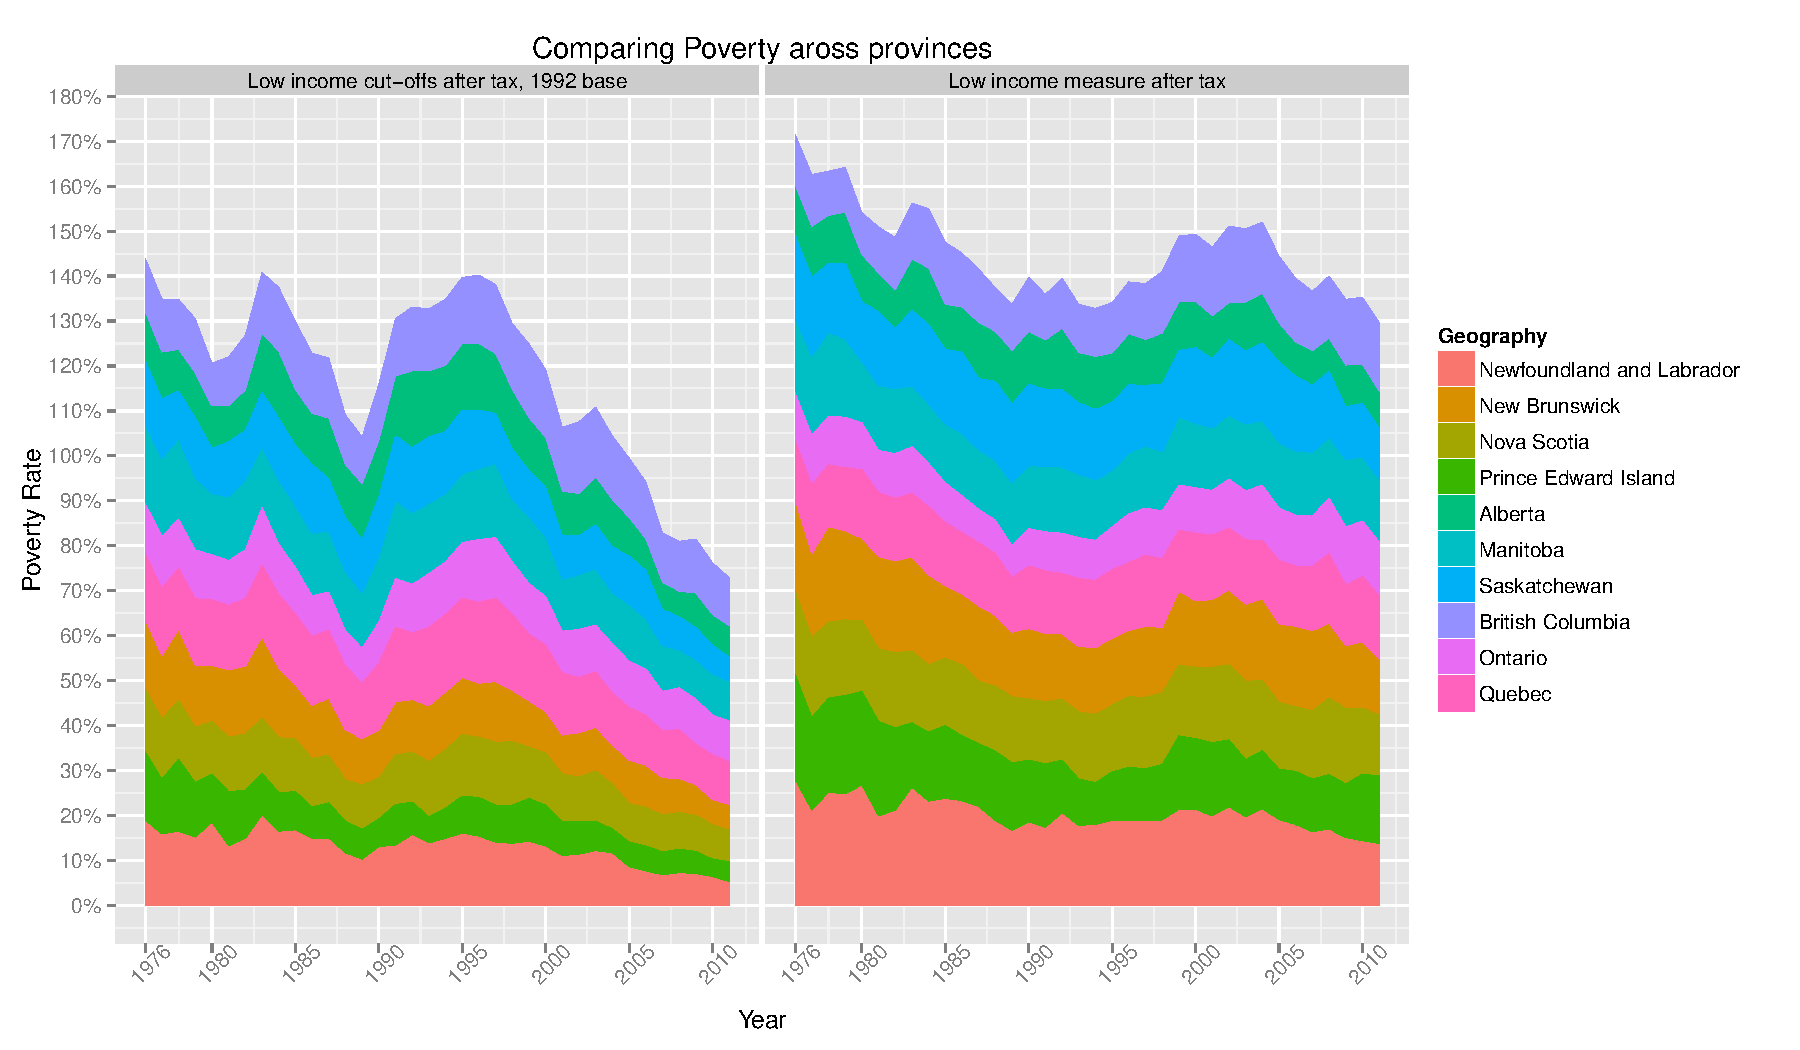
\includegraphics[width=\maxwidth]{figure/unnamed-chunk-17} 

\end{knitrout}

\end{center}
\end{figure}
\begin{figure}[ht]
\begin{center}
\begin{knitrout}
\definecolor{shadecolor}{rgb}{0.969, 0.969, 0.969}\color{fgcolor}
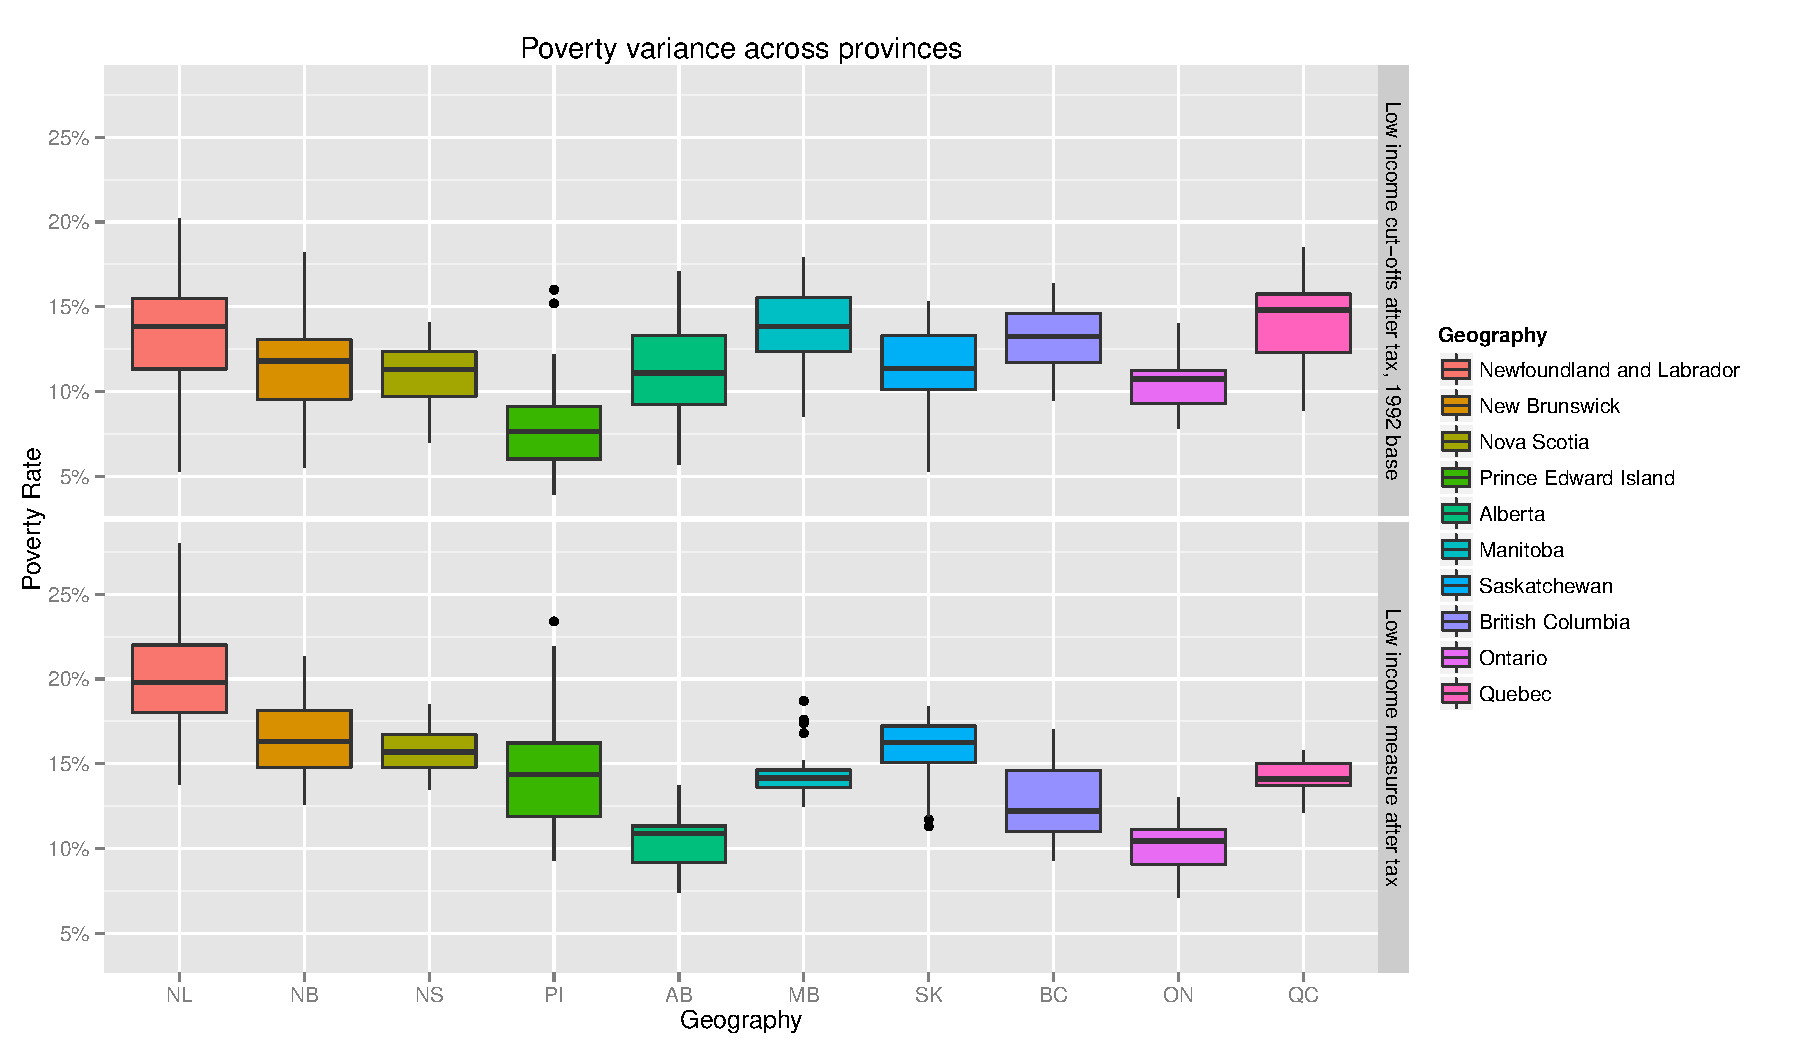
\includegraphics[width=\maxwidth]{figure/unnamed-chunk-18} 

\end{knitrout}

\end{center}
\end{figure}
\begin{figure}[ht]
\begin{center}
\begin{knitrout}
\definecolor{shadecolor}{rgb}{0.969, 0.969, 0.969}\color{fgcolor}
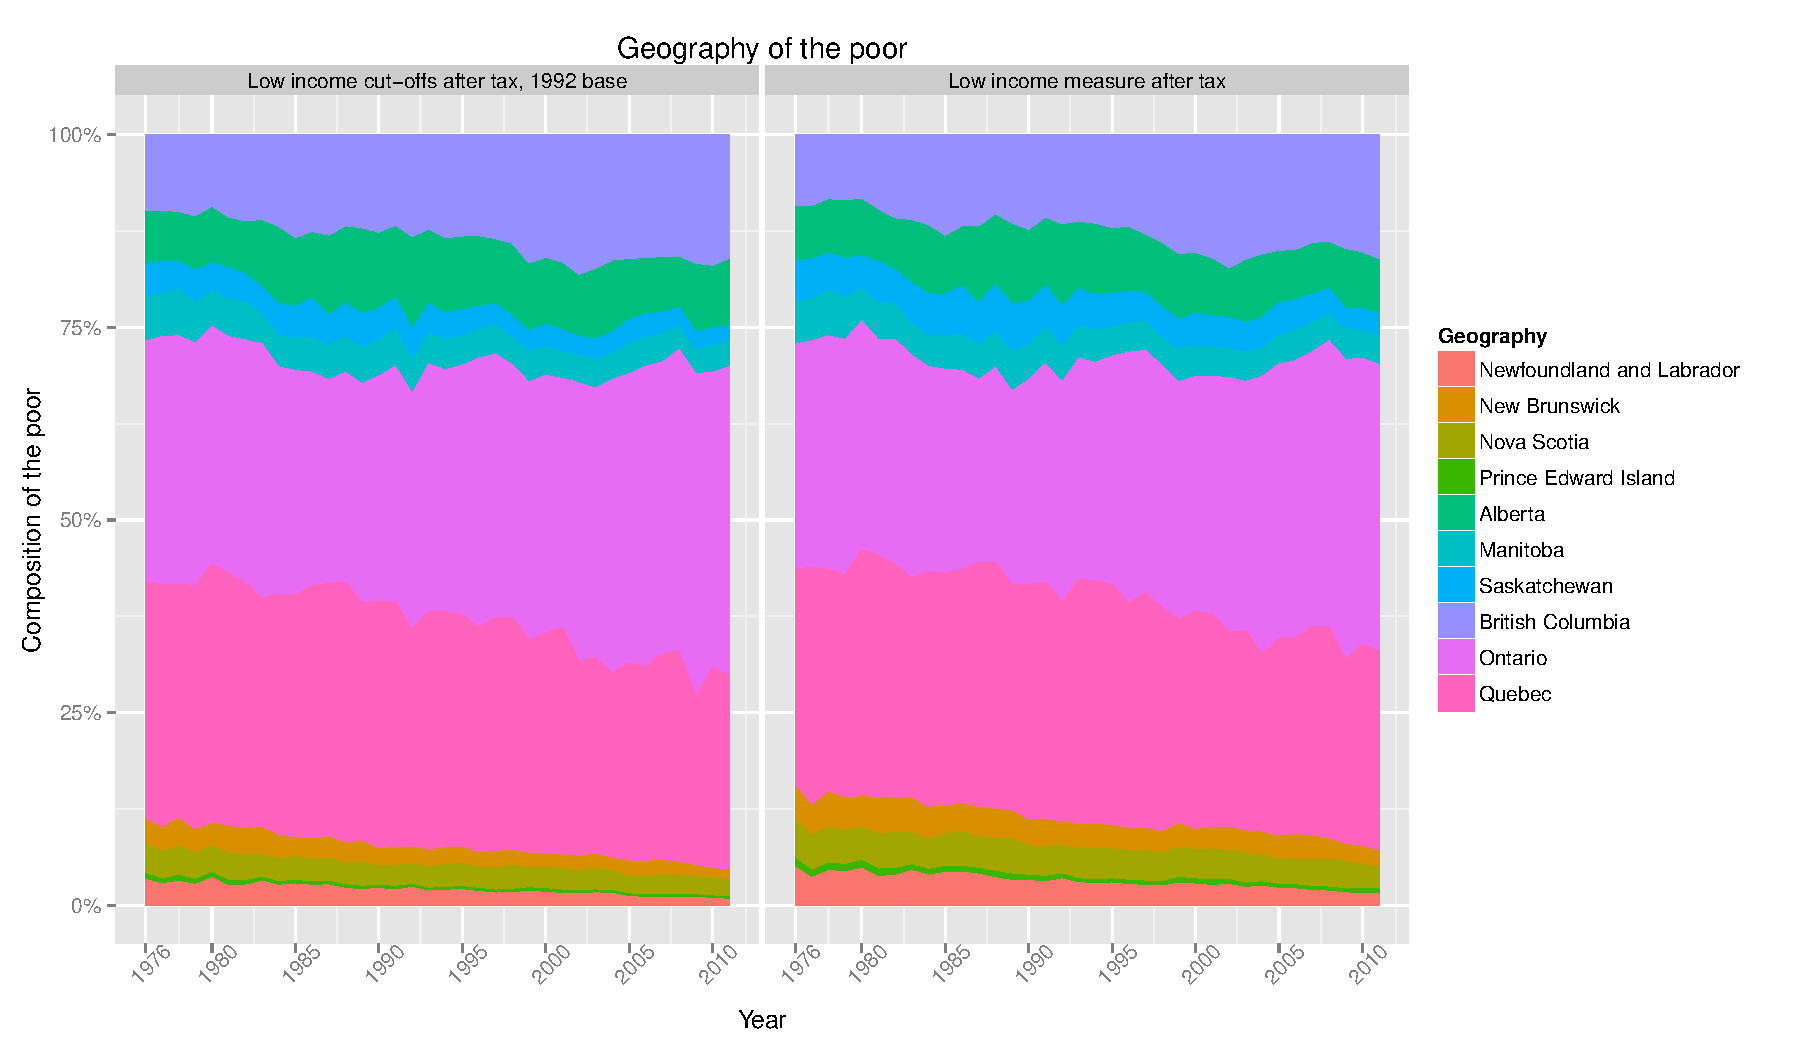
\includegraphics[width=\maxwidth]{figure/unnamed-chunk-19} 

\end{knitrout}

\end{center}
\end{figure}
\begin{figure}[ht]
\begin{center}
\begin{knitrout}
\definecolor{shadecolor}{rgb}{0.969, 0.969, 0.969}\color{fgcolor}
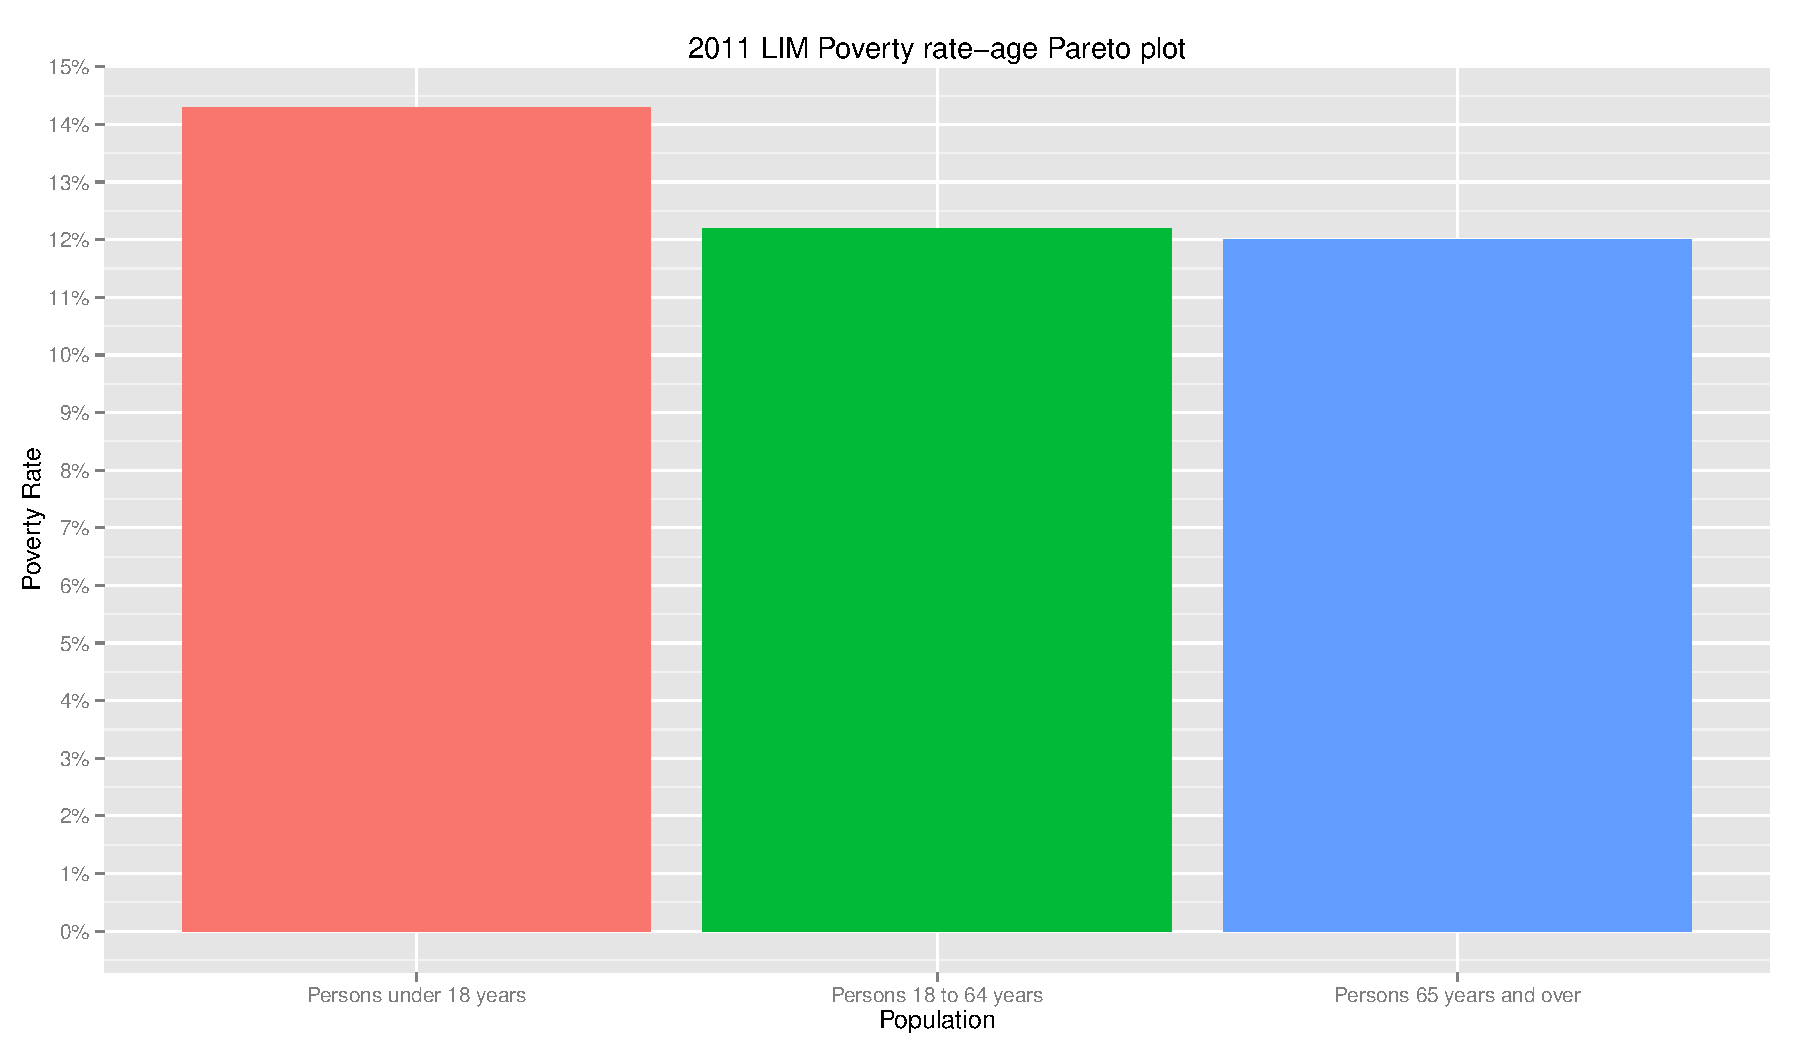
\includegraphics[width=\maxwidth]{figure/unnamed-chunk-20} 

\end{knitrout}

\end{center}
\end{figure}
\begin{figure}[ht]
\begin{center}
\begin{knitrout}
\definecolor{shadecolor}{rgb}{0.969, 0.969, 0.969}\color{fgcolor}
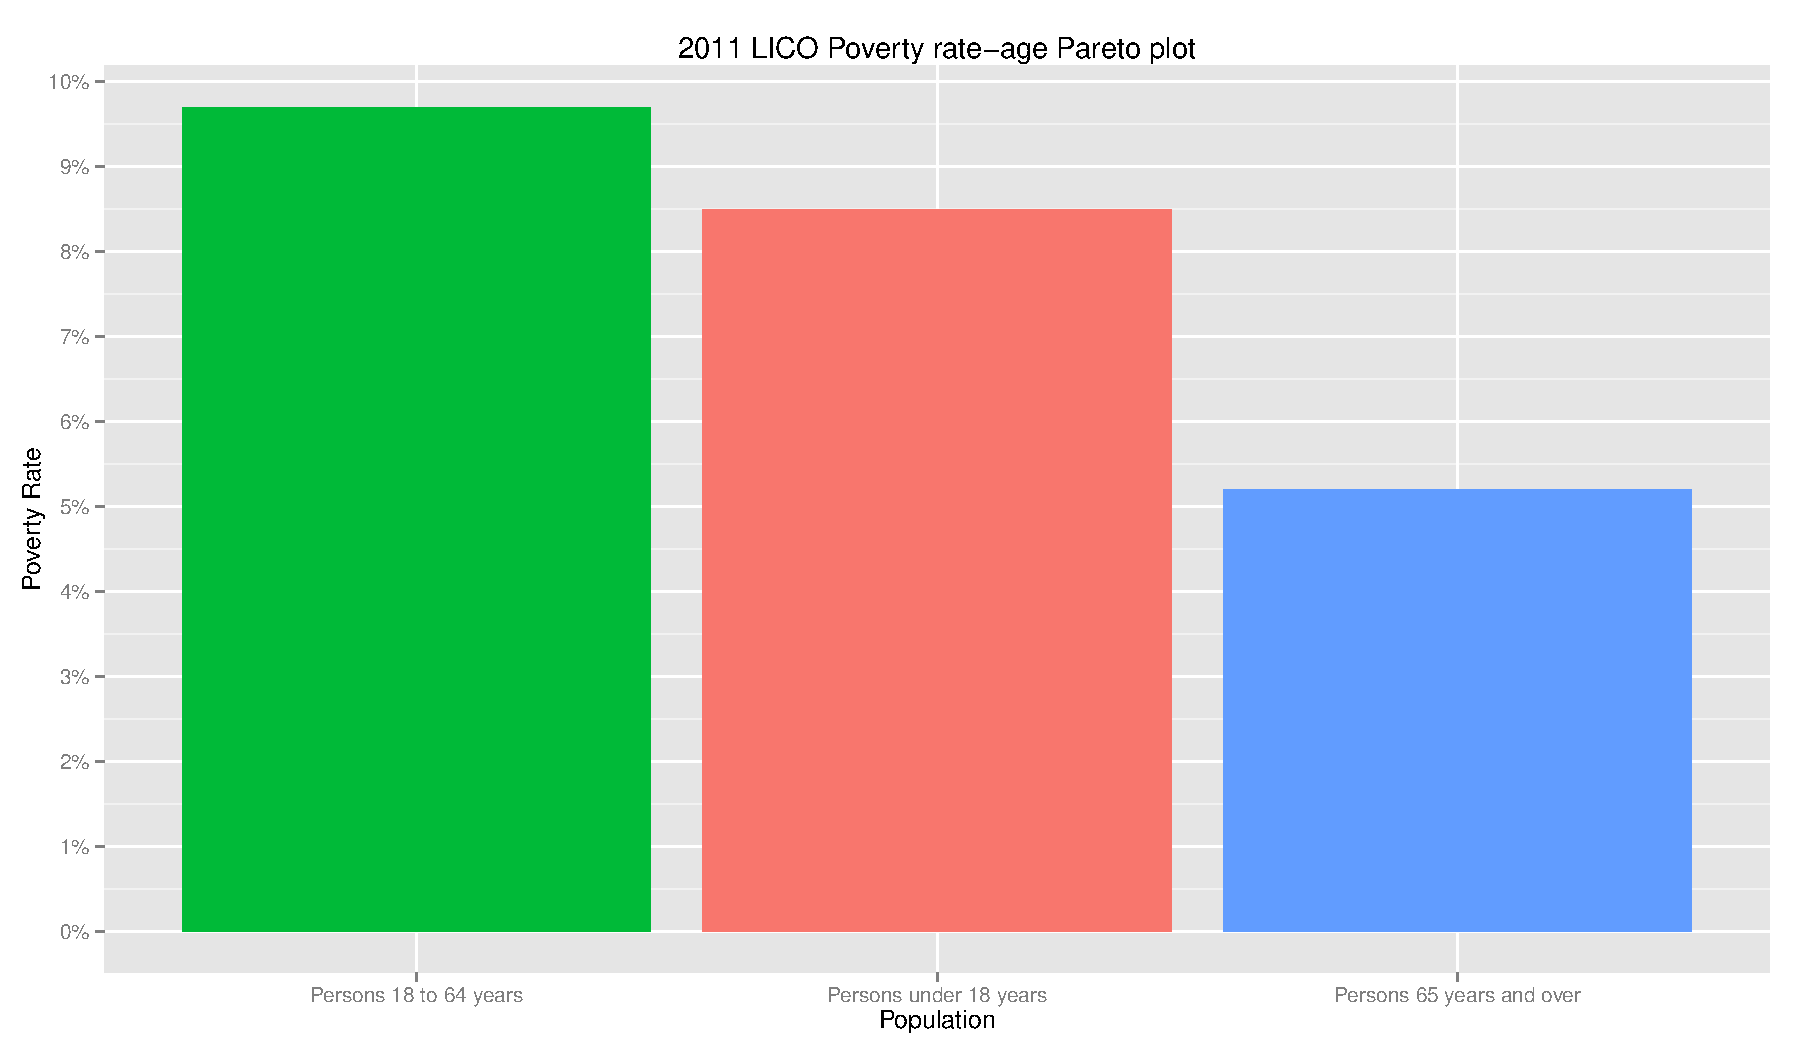
\includegraphics[width=\maxwidth]{figure/unnamed-chunk-21} 

\end{knitrout}

\end{center}
\end{figure}
\begin{figure}[ht]
\begin{center}
\begin{knitrout}
\definecolor{shadecolor}{rgb}{0.969, 0.969, 0.969}\color{fgcolor}
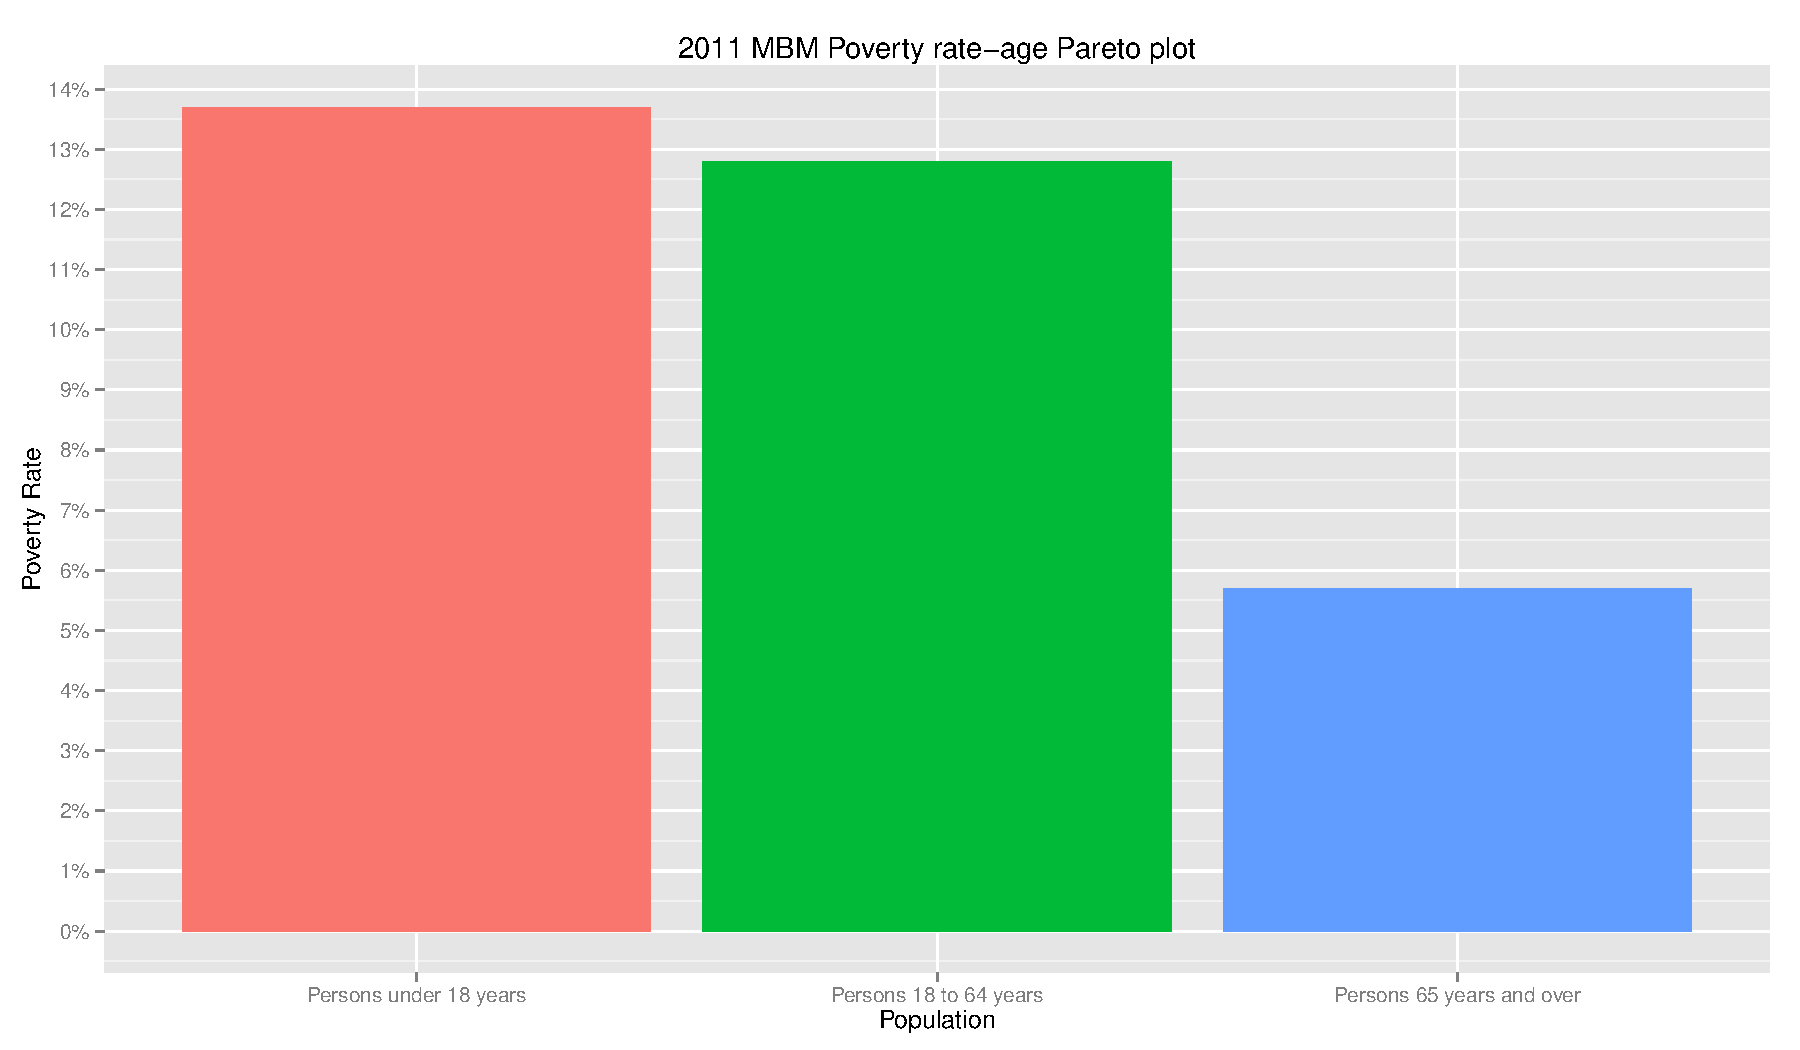
\includegraphics[width=\maxwidth]{figure/unnamed-chunk-22} 

\end{knitrout}

\end{center}
\end{figure}
\begin{figure}[ht]
\begin{center}
\begin{knitrout}
\definecolor{shadecolor}{rgb}{0.969, 0.969, 0.969}\color{fgcolor}
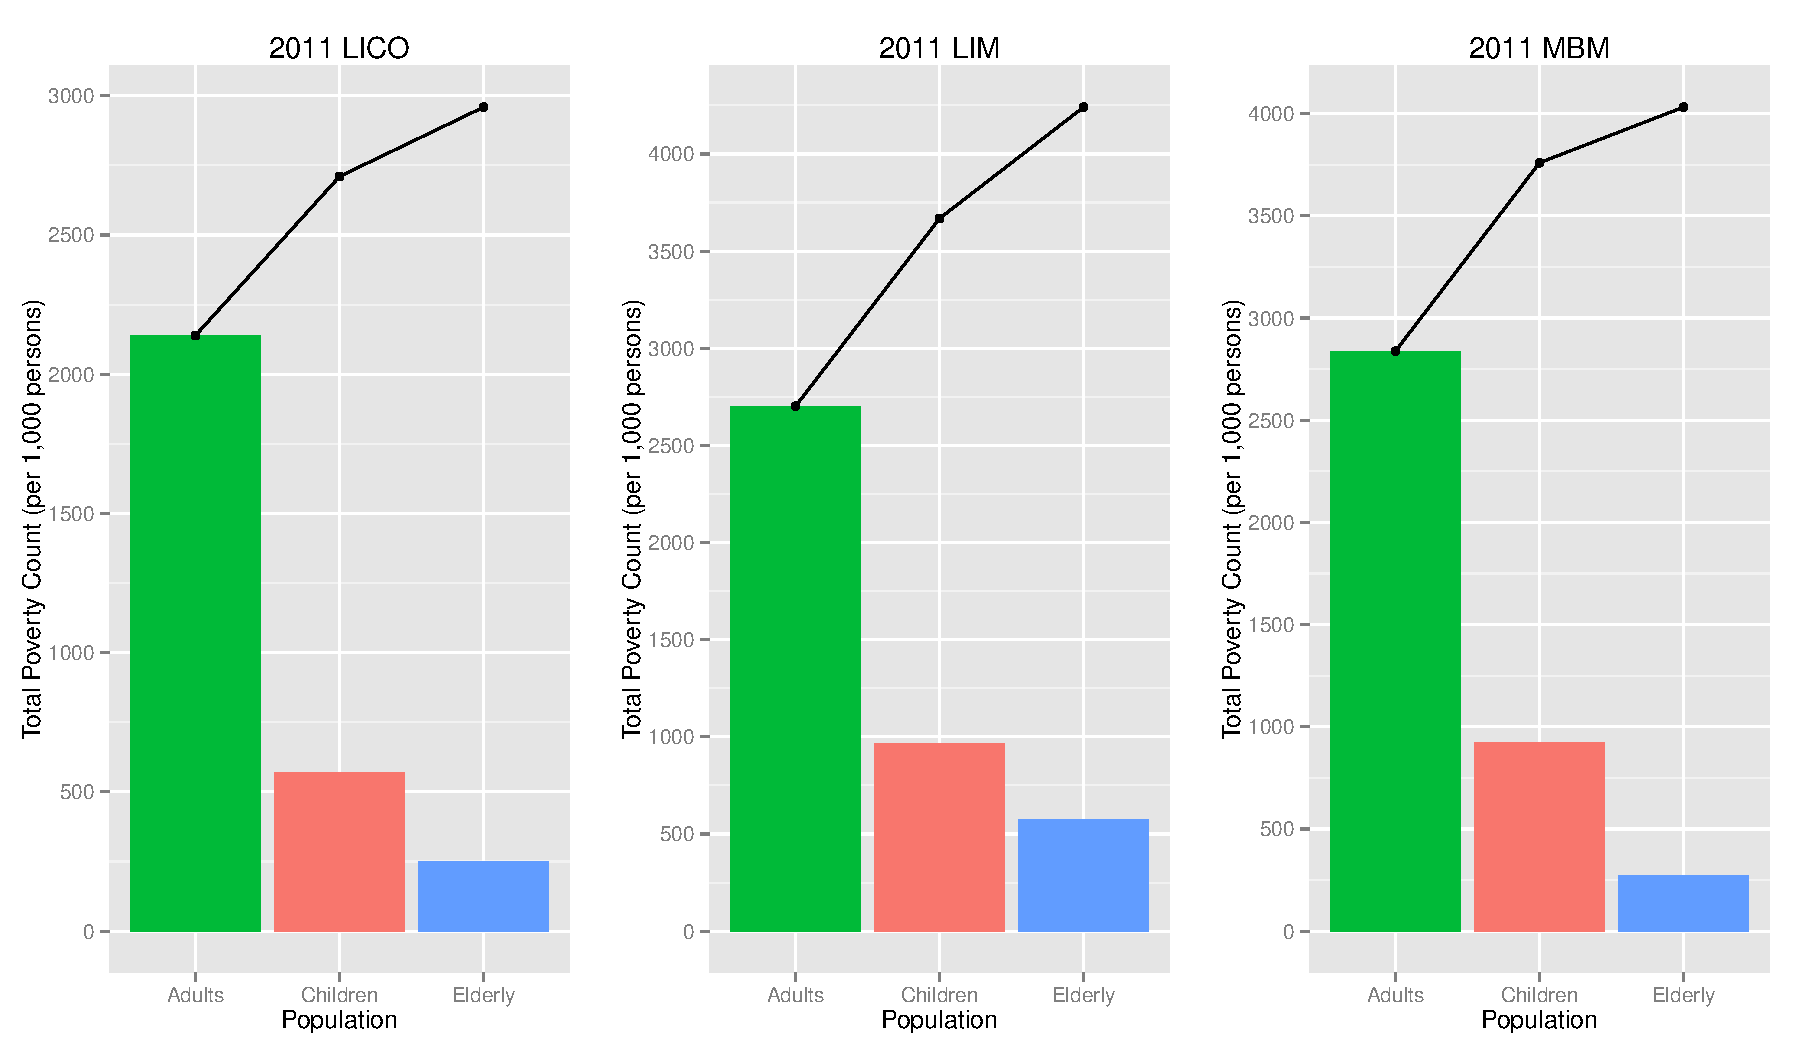
\includegraphics[width=\maxwidth]{figure/unnamed-chunk-23} 

\end{knitrout}

\end{center}
\end{figure}
\begin{figure}[ht]
\begin{center}
\begin{knitrout}
\definecolor{shadecolor}{rgb}{0.969, 0.969, 0.969}\color{fgcolor}
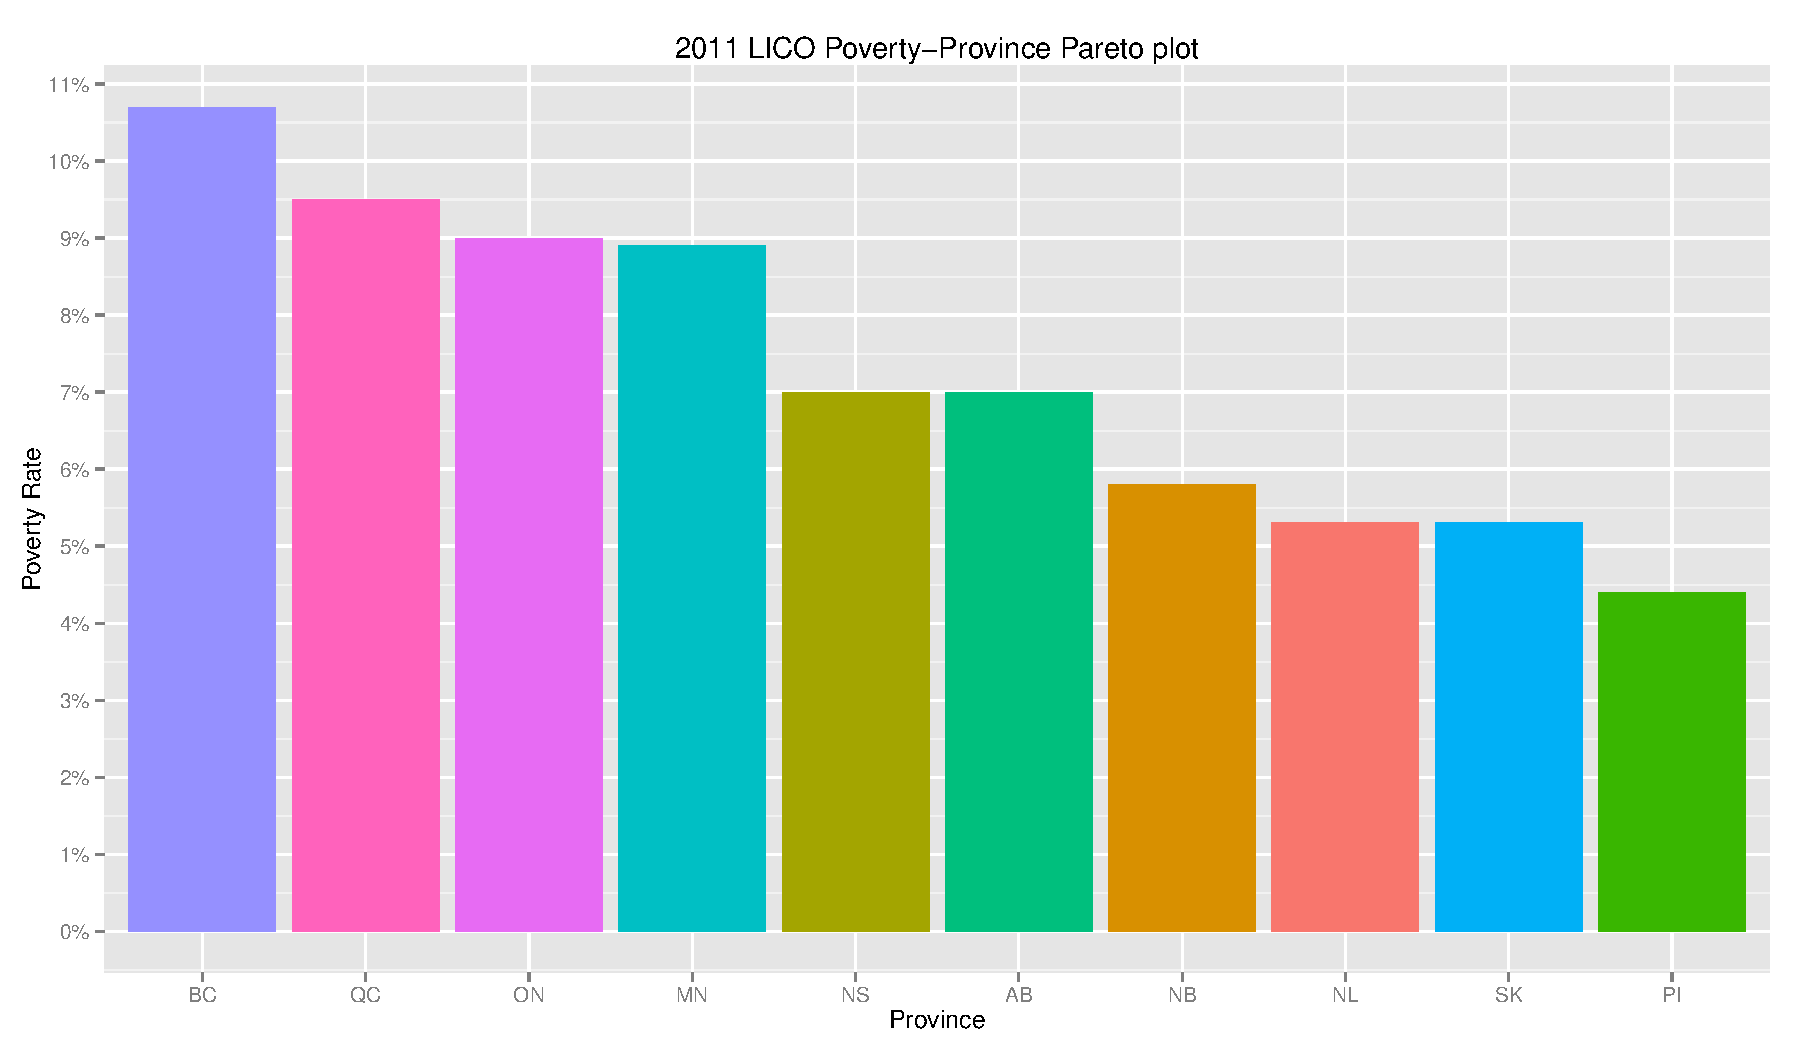
\includegraphics[width=\maxwidth]{figure/unnamed-chunk-24} 

\end{knitrout}

\end{center}
\end{figure}
\begin{figure}[ht]
\begin{center}
\begin{knitrout}
\definecolor{shadecolor}{rgb}{0.969, 0.969, 0.969}\color{fgcolor}
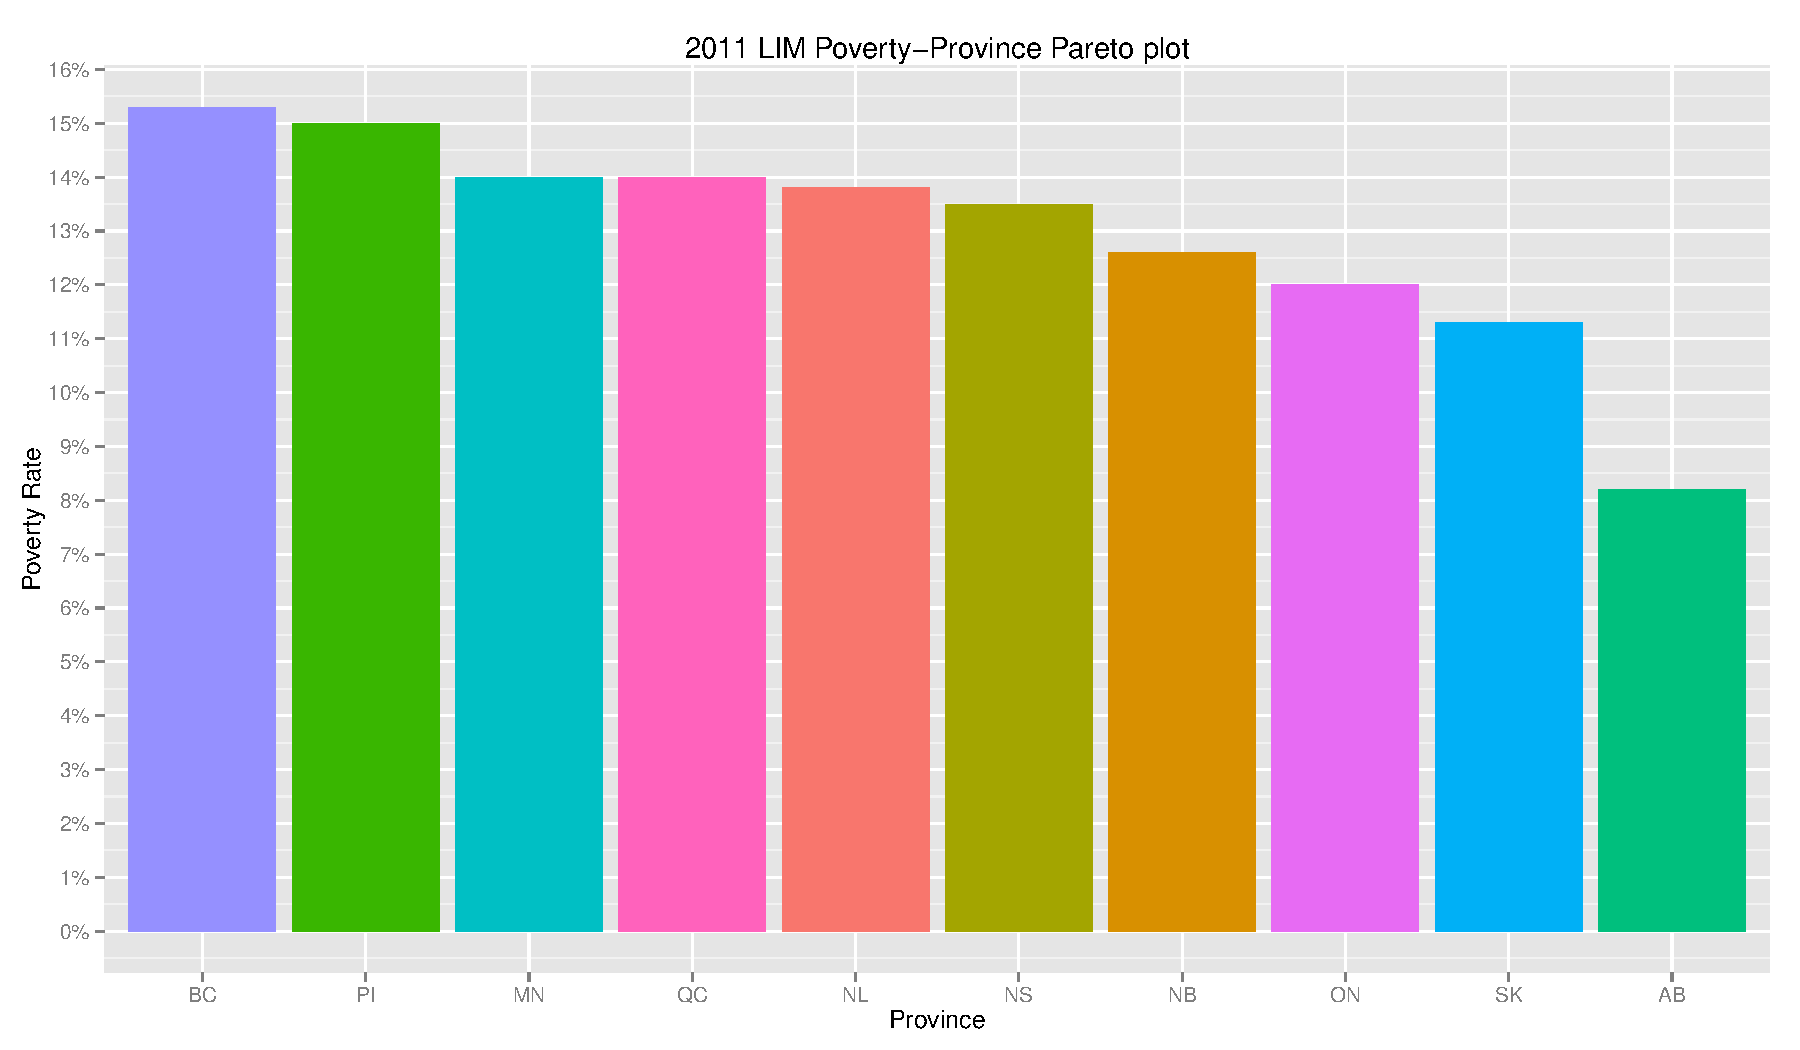
\includegraphics[width=\maxwidth]{figure/unnamed-chunk-25} 

\end{knitrout}

\end{center}
\end{figure}
\begin{figure}[ht]
\begin{center}
\begin{knitrout}
\definecolor{shadecolor}{rgb}{0.969, 0.969, 0.969}\color{fgcolor}
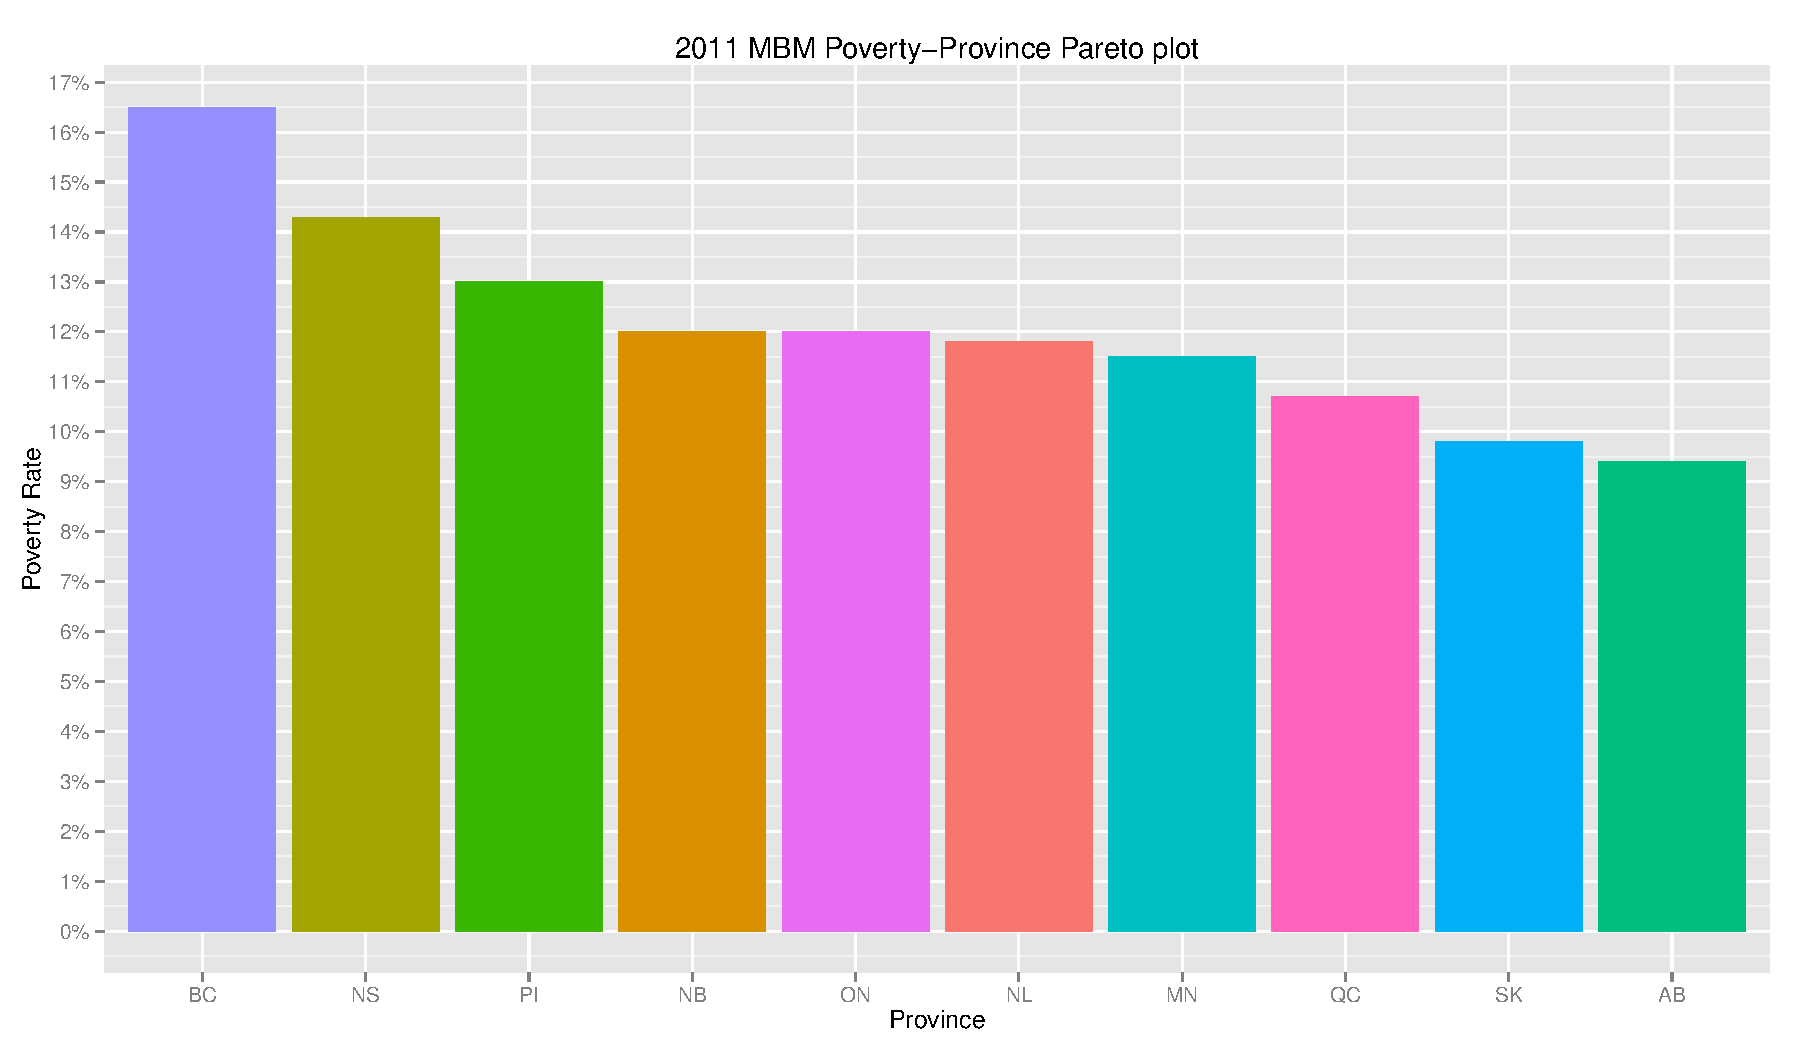
\includegraphics[width=\maxwidth]{figure/unnamed-chunk-26} 

\end{knitrout}

\end{center}
\end{figure}
\begin{figure}[ht]
\begin{center}
\begin{knitrout}
\definecolor{shadecolor}{rgb}{0.969, 0.969, 0.969}\color{fgcolor}
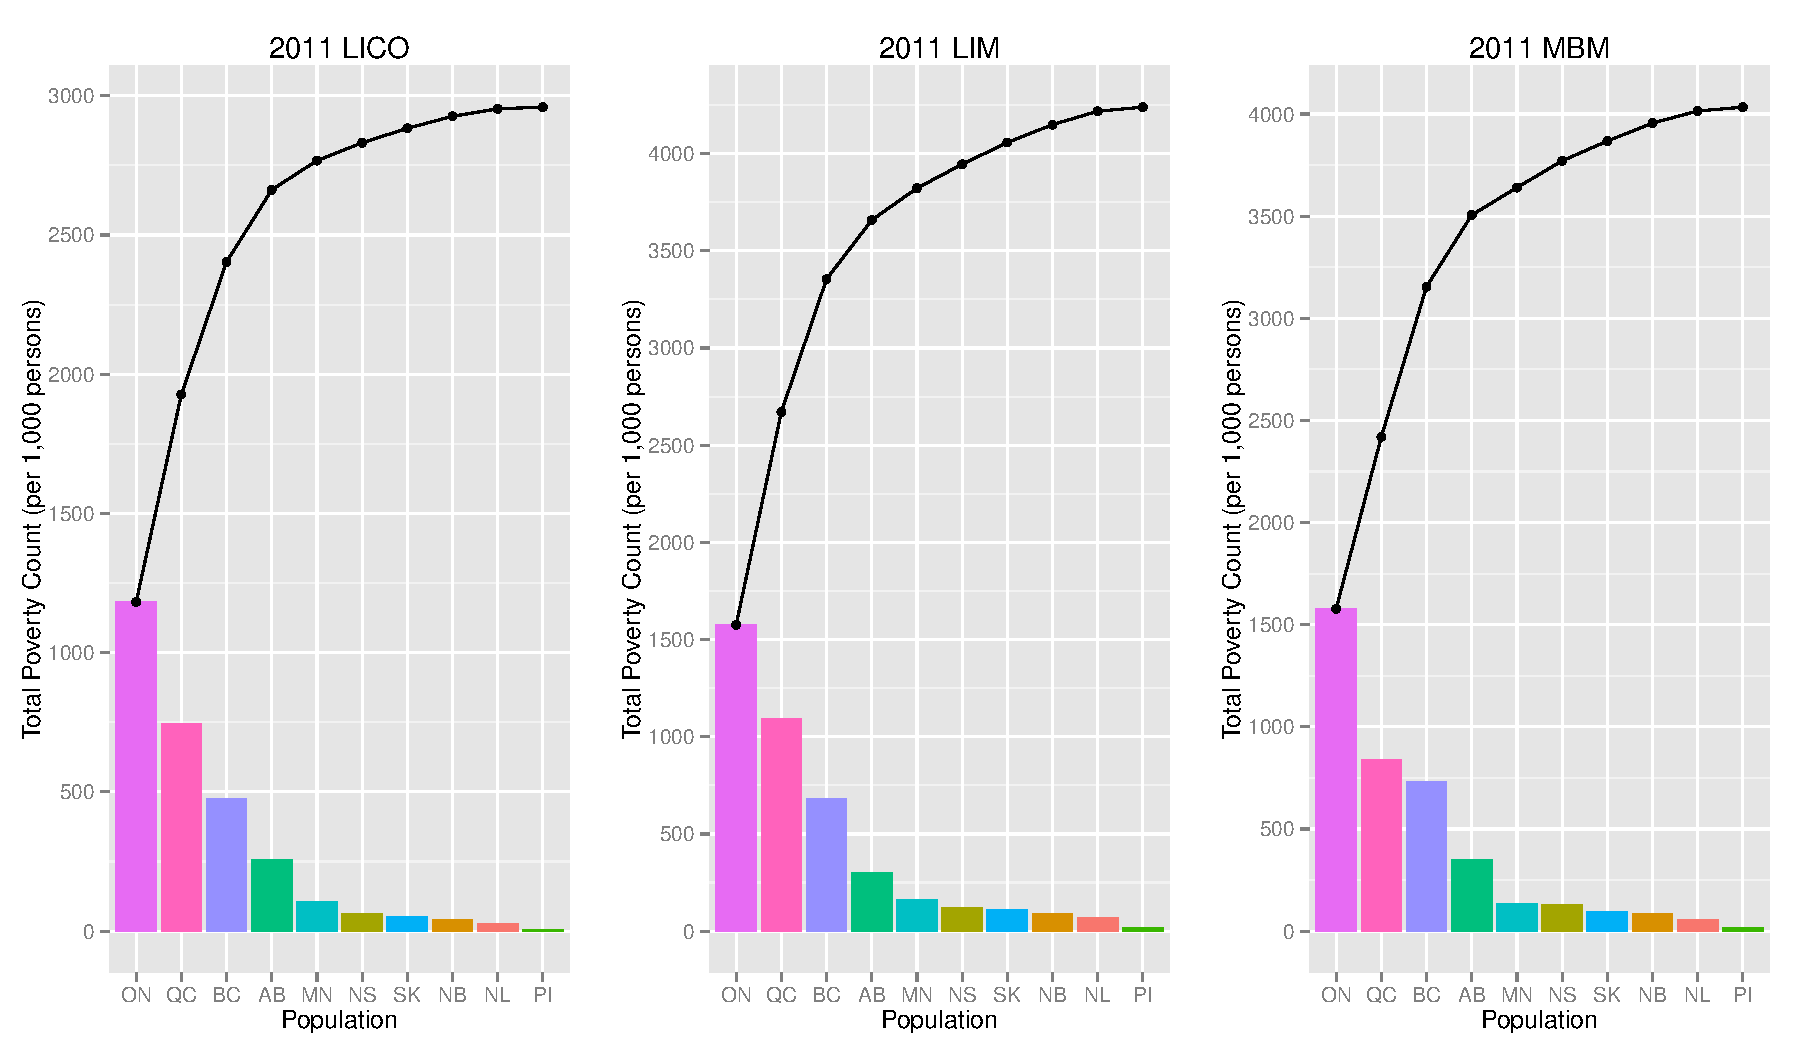
\includegraphics[width=\maxwidth]{figure/unnamed-chunk-27} 

\end{knitrout}

\end{center}
\end{figure}
\end{document}
